\section{\large{DESARROLLO}}
\vspace{-0.5cm}
\justifying

\subsection{\textbf{Sistema de control PID}}
\vspace{-0.5cm}
Para obtener una tensión de salida constante, sin importar variaciones en la tensión de entrada del
convertidor, o en la impedancia de la carga, se implementa un controlador PID.

\begin{figure}[H]
    \centering
    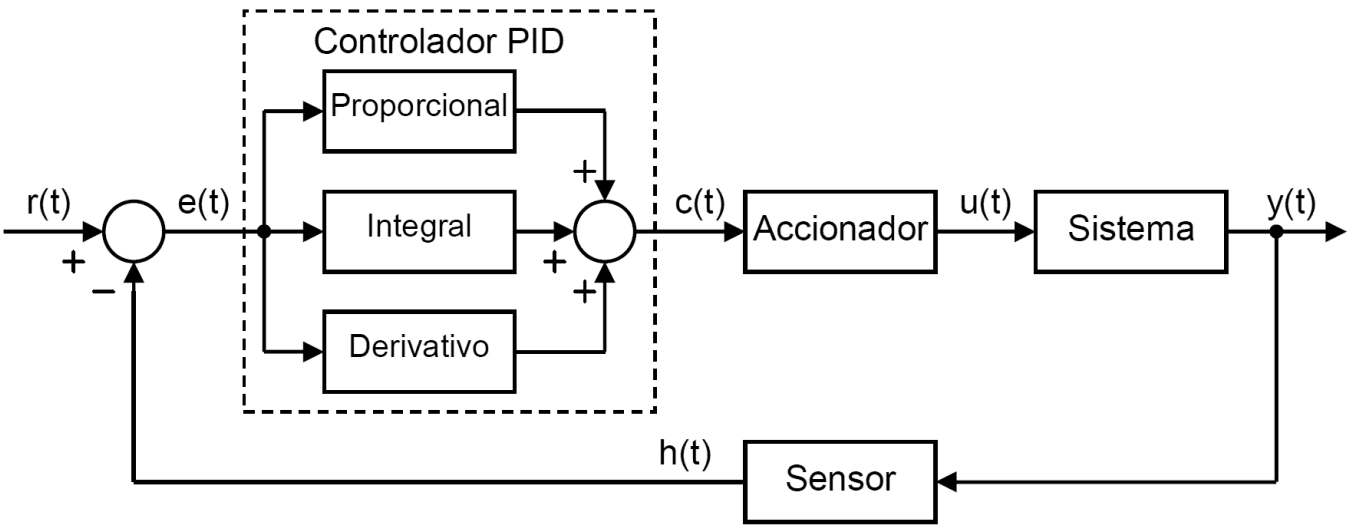
\includegraphics[height=4.5cm]{pid_diagrama.png}
    \vspace{-0.25cm}
    \caption{Diagrama de un sistema de control PID. \parencite{PICUINO}}
    \label{fig:pid_diagrama}
\end{figure}
\vspace{-0.5cm}

Donde:
\begin{itemize}[noitemsep]
    \item $r(t)$ es la señal de referencia, que indica el valor deseado a la salida del sistema.
    \item $h(t)$ es la señal de retroalimentación, que es la medición de un sensor de la salida del sistema.
    \item $e(t)$ es la señal de error, que es la diferencia entre la señal de referencia y la señal de
          retroalimentación del sistema.
    \item $c(t)$ es la señal de control, que es la salida del controlador PID.
    \item $u(t)$ es la señal de entrada al sistema.
    \item $y(t)$ es la salida del sistema.
\end{itemize}

El controlador PID consiste de tres acciones de control diferentes, que se suman para poder
obtener la señal de control. Estas acciones son:

\textbf{Acción de control proporcional (P):} es simplemente la multiplicación de la señal de error por
una constante $K_p$. Esto significa que su acción es proporcional al error. Su función de transferencia es:

\vspace{-0.5cm}
\begin{equation}
    \dfrac{U(s)}{E(s)} = K_p
\end{equation}
\vspace{-0.5cm}

\textbf{Acción de control integral (I):} es la suma acumulada de la señal de error en el tiempo, multiplicada
por una constante $K_i$. Su función de transferencia es:

\vspace{-0.5cm}
\begin{equation}
    \dfrac{U(s)}{E(s)} = \dfrac{K_i}{s}
\end{equation}
\vspace{-0.5cm}

\textbf{Acción de control derivativa (D):} es la derivada de la señal de error en el tiempo, multiplicada por
una constante $K_d$. Su función de transferencia es:

\vspace{-0.5cm}
\begin{equation}
    \dfrac{U(s)}{E(s)} = K_d \cdot s
\end{equation}
\vspace{-0.5cm}

Para reducir el ruido de alta frecuencia en la señal de control, así como para evitar inestabilidades
en el sistema, se utiliza un filtro pasa-bajos en la acción derivativa. La función de transferencia es:

\vspace{-0.5cm}
\begin{equation}
    \dfrac{U(s)}{E(s)} = K_d \cdot \dfrac{N}{1+\dfrac{N}{s}}
\end{equation}
\vspace{-0.5cm}

Sumando las tres acciones de control, obtenemos la función de transferencia en forma paralela del controlador PID:

\vspace{-0.5cm}
\begin{equation}
    \dfrac{U(s)}{E(s)} = K_p + \dfrac{K_i}{s} + K_d \cdot \dfrac{N}{1+\dfrac{N}{s}}
\end{equation}
\vspace{-0.5cm}

Como en nuestro sistema de control se utiliza un microcontrolador, se debe discretizar la función de transferencia
del controlador PID para implementarla correctamente. Utilizando la transformación de Euler, se obtiene la siguiente
función de transferencia discreta:

\vspace{-0.5cm}
\begin{equation}
    \dfrac{U(s)}{E(s)} = K_p + K_i \cdot \dfrac{T_s}{z-1} + K_d \cdot \dfrac{N}{1+N \cdot \dfrac{T_s}{z-1}}
\end{equation}
\vspace{-0.5cm}

Aplicando denominador común y agrupando términos, se obtiene:

\vspace{-0.5cm}
\begin{equation}
    \dfrac{U(z)}{E(z)} =
    \frac
    {
        \splitfrac{
            (K_p + K_d N)\ z^2 + (-2 K_p - 2 K_d N + K_i T_s + K_p N T_s)\ z
        }{
            + (K_p + K_d N - K_i T_s - K_p N T_s + K_i N {T_s}^2)
        }
    }
    {
            z^2 + (-2 + N T_s) z + (1 - N T_s)
    }
    \end{equation}
\vspace{-0.5cm}

Finalmente, se puede obtener la ecuación en diferencias del controlador PID:

\vspace{-0.5cm}
\begin{multline}
        u[n] = (K_p + K_d N)\ e[n] + (-2 K_p - 2 K_d N + K_i T_s + K_p N T_s)\ e[n-1]\  + \\
    (K_p + K_d N - K_i T_s - K_p N T_s + K_i N {T_s}^2)\ e[n-2] - (-2 + N T_s)\ u[n-1] - (1 - N T_s)\ u[n-2]
\end{multline}
\vspace{-0.5cm}

\vspace{-0.5cm}
\subsection{\textbf{Modelado del sistema}}
\vspace{-0.5cm}

El sistema convertidor Buck es un sistema conmutado. Consta de dos estados de conmutación: 
en primer lugar, cuando el interruptor está conectado al nodo 1, estado de carga; en segundo lugar, cuando
el interruptor está conectado al nodo 2, estado de descarga.
El sistema conmutado se puede modelar como un sistema promediado.

\begin{figure}[H]
    \centering
    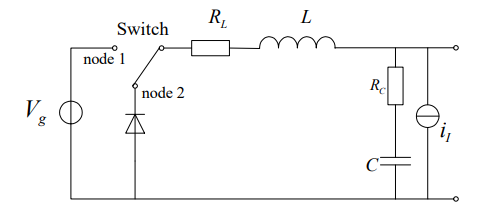
\includegraphics[height=4.5cm]{modelado_circuito.png}
    \vspace{-0.25cm}
    \caption{Circuito general del sistema.}
    \label{fig:modelado_circuito}
\end{figure}
\vspace{-0.5cm}

Primero, la fuente se incluye en el circuito cuando el interruptor está conectado al nodo 1.

\begin{figure}[H]
    \centering
    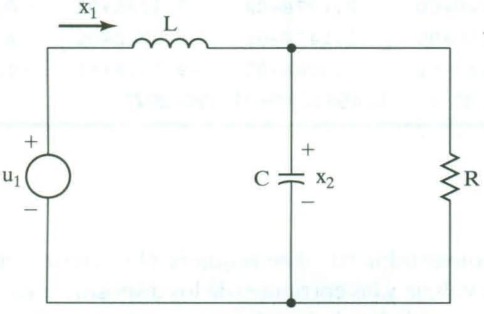
\includegraphics[height=4.5cm]{modelo_con_vg.png}
    \vspace{-0.25cm}
    \caption{Circuito con fuente de voltaje.}
    \label{fig:modelado_con_vg}
\end{figure}
\vspace{-0.5cm}

Aplicando ley de Kirchoff obtenemos:

\vspace{-0.5cm}
\begin{equation}
    u_1 = Lx'_1 + x_2
\end{equation}

\vspace{-0.5cm}
\begin{equation}
    Cx'_2 = x_1 - \dfrac{1}{R} x_2 
\end{equation}

Donde $x_1$ es la corriente que circula por el inductor, $x_2$ es la tensión en el capacitor y $u_1$ la tensión de entrada.
Reordenando nos queda:

\vspace{-0.5cm}
\begin{equation}
    x'_1 = -\dfrac{1}{L} x_2 + \dfrac{1}{L} u_1
\end{equation}

\vspace{-0.5cm}
\begin{equation}
    x'_2 = \dfrac{1}{C}x_1 - \dfrac{1}{RC} x_2 
\end{equation}

De aquí podemos obtener las matrices $A_1$ y $B_1$:

\begin{equation}
    A_1 = \begin{bmatrix}
        0 & -\dfrac{1}{L}\\
        \\
        \dfrac{1}{C} & -\dfrac{1}{RC}
    \end{bmatrix}
\end{equation}

\vspace{-0.5cm}
\begin{equation}
    B_1 = \begin{bmatrix}
        \dfrac{1}{L}\\
        \\
        0
    \end{bmatrix}
\end{equation}

Cuando el interruptor está conectado al nodo dos, la fuente de tensión 
no se incluye en el circuito.

\begin{figure}[H]
    \centering
    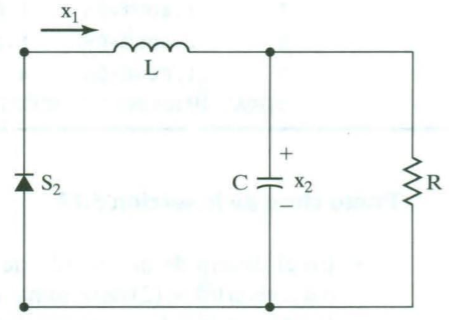
\includegraphics[height=4.5cm]{modelo_sin_vg.png}
    \vspace{-0.25cm}
    \caption{Circuito sin fuente de voltaje.}
    \label{fig:modelado_sin_vg}
\end{figure}
\vspace{-0.5cm}

Nuevamente aplicando ley de Kirchoff, y reordenando las ecuaciones:

\vspace{-0.75cm}
\begin{equation}
    0 = Lx'_1 + x_2
\end{equation}

\vspace{-0.75cm}
\begin{equation}
    Cx'_2 = x_1 - \dfrac{1}{R} x_2 
\end{equation}

\vspace{-0.75cm}
\begin{equation}
    x'_1 = -\dfrac{1}{L} x_2
\end{equation}

\vspace{-0.75cm}
\begin{equation}
    x'_2 = \dfrac{1}{C} x_1 - \dfrac{1}{RC} x_2 
\end{equation}

De aquí podemos obtener las matrices $A_2$ y $B_2$:

\begin{equation}
    A_2 = \begin{bmatrix}
        0 & -\dfrac{1}{L}\\
        \\
        \dfrac{1}{C} & -\dfrac{1}{RC}
    \end{bmatrix}
\end{equation}

\vspace{-0.5cm}
\begin{equation}
    B_2 = \begin{bmatrix}
        0\\
        0
    \end{bmatrix}
\end{equation}

Para los dos casos, la salida es igual a la tensión en el capacitor, $x_2$:

\vspace{-0.5cm}
\begin{equation}
    y = \begin{bmatrix}
        0 & 1
    \end{bmatrix}
    \cdot
    \begin{bmatrix}
        x_1 \\
        x_2
    \end{bmatrix}
\end{equation}

\textbf{Obtención del sistema promediado:} la solución total se puede obtener promediando en espacio de estados, esto es, sumando los términos 
para cada análisis del modo lineal conmutado. Como solo cambia la matriz B, se hace sobre esa única matriz.
Suponiendo el ciclo de trabajo d, tenemos:

\vspace{-0.5cm}
\begin{equation}
    B_{Promedio} = d \cdot B_1 + (1 - d) \cdot B_2
\end{equation}

Sustituyendo obtenemos la matriz A, B y C del sistema:

\begin{equation}
    A = \begin{bmatrix}
        0 & -\dfrac{1}{L}\\
        \\
        \dfrac{1}{C} & -\dfrac{1}{RC}
    \end{bmatrix}
\end{equation}

\vspace{-0.5cm}
\begin{equation}
    B = \begin{bmatrix}
        \dfrac{d}{L}\\
        \\
        0
    \end{bmatrix}
\end{equation}

\vspace{-0.5cm}
\begin{equation}
    C = \begin{bmatrix}
        0 & 1
    \end{bmatrix}
\end{equation}

Lo que resulta en el siguiente sistema de estado:

\vspace{-0.5cm}
\begin{equation}
    \begin{cases}
        \begin{bmatrix}
            \dot{x_1}\\
            \dot{x_2}
        \end{bmatrix}
        =
        \begin{bmatrix}
            0  &   -\dfrac{1}{L}\\
            \\
            \dfrac{1}{C} & -\dfrac{1}{RC}
        \end{bmatrix}
        \cdot
        \begin{bmatrix}
            x_1 \\
            x_2
        \end{bmatrix}
        +
        \begin{bmatrix}
            \dfrac{d}{L} \\
            \\
            0
        \end{bmatrix}
        \cdot
        u_1 
        \\
        \\
        y =
        \begin{bmatrix}
            0 & 1
        \end{bmatrix}
        \cdot
        \begin{bmatrix}
            x_1 \\
            x_2
        \end{bmatrix}

    \end{cases}
\end{equation}

Aunque el sistema original es lineal para toda condición dada de conmutación, el sistema que resulta 
en general es no lineal debido a que el ciclo de trabajo d es en general una función de $x_1$, $x_2$ y $u_1$. \parencite{RASHID}

Se procede a implementar el circuito físico para luego obtener un modelo del sistema lineal e invariable en el tiempo mediante
identificación empírica.

\vspace{-0.5cm}
\subsection{\textbf{Circuito}}
\vspace{-0.5cm}

Para construir el circuito físico, primero se realizó el siguiente diagrama:

\begin{figure}[H]
    \centering
    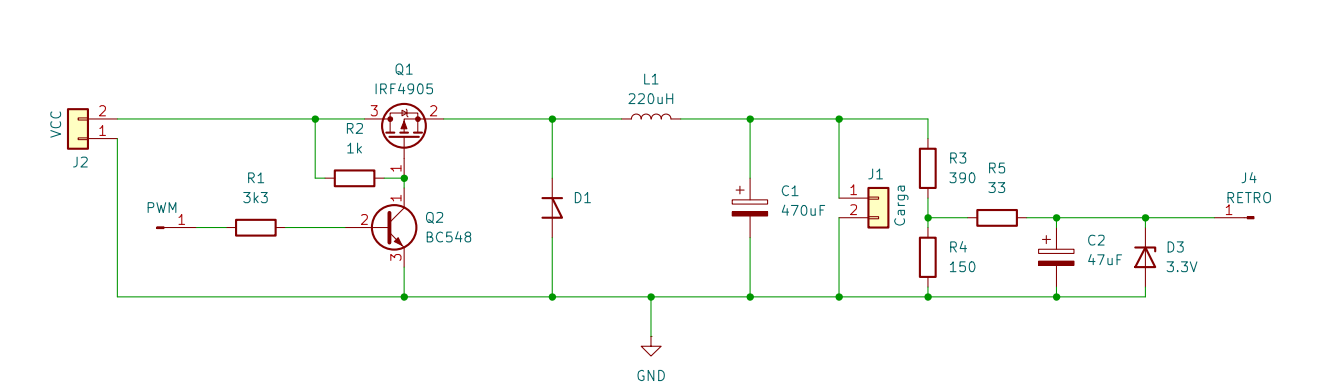
\includegraphics[width=\textwidth]{diagrama_circuito.png}
    \vspace{-0.25cm}
    \caption{Diagrama de circuito.}
    \label{fig:diagrama_circuito}
\end{figure}
\vspace{-0.5cm}

Los componentes fueron seleccionados según disponibilidad y costos, teniendo en cuenta que cumplan los requerimientos del circuito.
El IRF4905 es un transistor MOSFET canal P que se utiliza como interruptor en el convertidor. Su baja resistencia Rds(on) cuando está activado y 
su capacidad para manejar corrientes altas lo hacen adecuado para aplicaciones de conversión de potencia.

El filtro LC se diseña para rechazar la frecuencia de conmutación del transistor (establecida arbitrariamente en 19 kHz),
resultando en una frecuencia de corte de 770 Hz. Además, se coloca un filtro RC a la salida de la retroalimentación, con una frecuencia
de corte de 100 Hz para filtrar cualquier dinámica indeseada del sistema que no haya sido eliminada por el filtro LC. 

El divisor resistivo que conecta la retroalimentación al microcontrolador está diseñado para que entregue una 
tensión de 0 V a 3,3 V. Para ello se realizó una tabla con valores de entrada y salida:

\begin{table}[H]
    \centering
    \begin{tabular}{|c|c|}
    \hline
    Voltaje de retroalimentación (V) & Voltaje en la carga (V) \\ \hline
    0                                & 0                       \\
    0,27                             & 1                       \\
    0,55                             & 2                       \\
    0,83                             & 3,05                    \\
    1,07                             & 3,9                     \\
    1,38                             & 5,01                    \\
    1,66                             & 6,03                    \\
    1,95                             & 7,09                    \\
    2,19                             & 8,02                    \\
    2,44                             & 9,06                    \\
    2,65                             & 9,96                    \\
    2,87                             & 11                      \\
    3,04                             & 12                      \\ \hline
    \end{tabular}
    \label{tab:calibración_fb}
    \vspace{-0.25cm}
    \caption{Calibración de voltaje de retroalimentación}
\end{table}
\vspace{-0.75cm}

\begin{figure}[H]
    \centering
    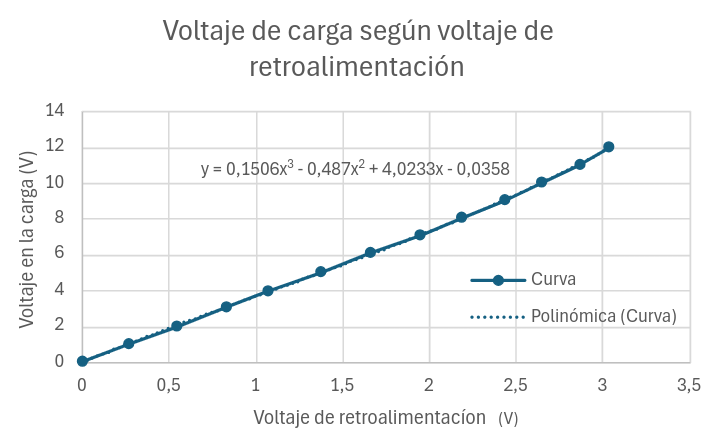
\includegraphics[height=6.5cm]{curva_calibracion.png}
    \vspace{-0.25cm}
    \caption{Curva de calibración de voltaje de retroalimentación.}
    \label{fig:calibracion}
\end{figure}
\vspace{-0.5cm}

\begin{figure}[H]
    \centering
    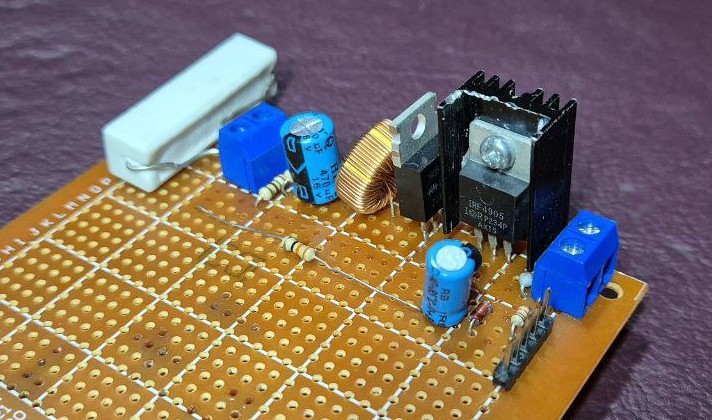
\includegraphics[height=6.5cm]{circuito.jpg}
    \vspace{-0.25cm}
    \caption{Circuito montado en placa perforada, con carga resistiva montada.}
    \label{fig:circuito}
\end{figure}
\vspace{-0.5cm}

\vspace{-0.5cm}
\subsection{\textbf{Identificación del sistema}}
\vspace{-0.5cm}
Si bien el modelo del sistema se puede obtener a partir de las ecuaciones de Kirchhoff, se procede
a obtener un modelo empírico. Para ello, se aplica una señal de entrada al sistema físico y se
mide la respuesta del mismo.

A fin de diseñar un modelo que sea efectivo en situaciones prácticas, primero se analiza la respuesta
del sistema, con distintos valores de ciclo de trabajo (duty):

\begin{figure}[H]
    \centering
    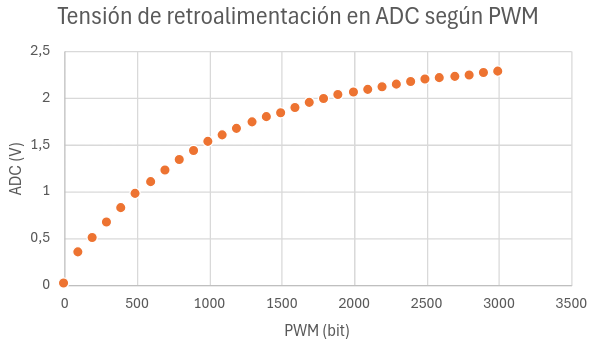
\includegraphics[height=6cm]{lineal.png}
    \vspace{-0.25cm}
    \caption{Respuesta del sistema ante distintos valores de duty.}
    \label{fig:lineal}
\end{figure}
\vspace{-0.5cm}

En esta ocasión, se optó por utilizar una señal de entrada PRBS
(Pseudo Random Binary Sequence, en español Secuencia Binaria Pseudo Aleatoria). La misma intenta
cubrir todo el rango de frecuencias posibles, y es útil para identificar sistemas lineales y no lineales.
Utilizando MATLAB, se genera una señal PRBS con un tiempo de muestreo de 200 microsegundos, frecuencia máxima
100 Hz, y una duración de 10 períodos. Esta señal es una secuencia de 750 valores en 0,15 segundos, repetida diez veces.
Es decir, 7500 valores en un rango de 0 a 1,5 segundos.

Se programa el microcontrolador para reproducir la señal PRBS en el convertidor Buck, medir la salida
del sistema y luego enviar los datos mediante comunicación serial. La identificación se realizó de tal manera 
que los valores de 0 en la señal PRBS signifiquen ciclo de trabajo 0, mientras que los valores de 1 sean ciclo
de trabajo 1000. A través de un programa en Python, se guardan los valores en un archivo csv para luego introducir en el
System Identification Toolbox de MATLAB:


\begin{figure}[H]
    \centering
    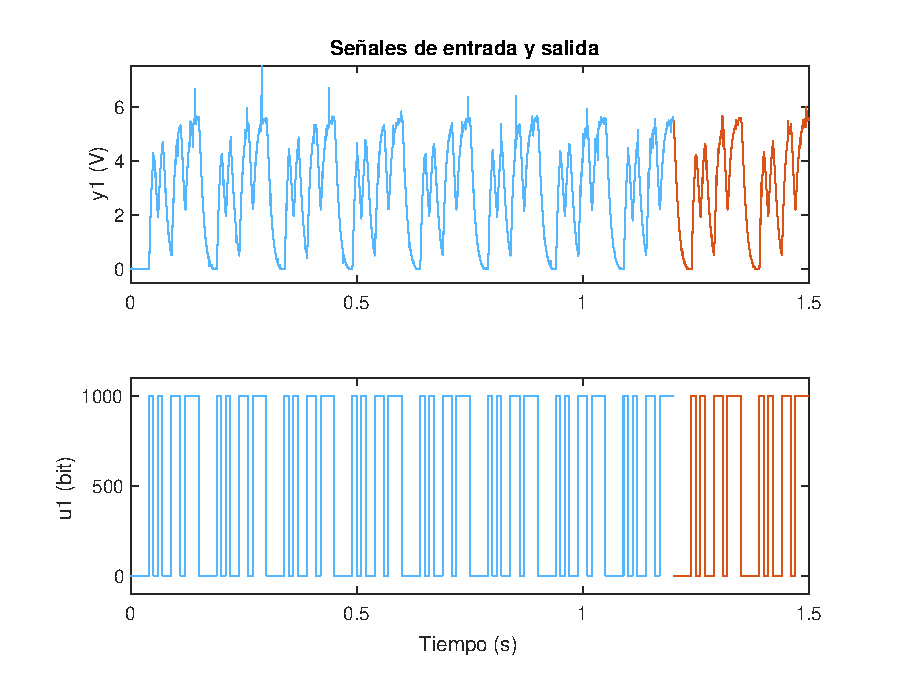
\includegraphics[height=8cm]{identificacion_io.eps}
    \vspace{-0.25cm}
    \caption{Salida (arriba) y entrada (abajo) del sistema con la señal de identificación.}
    \label{fig:identificacion_io}
\end{figure}
\vspace{-0.5cm}

Se seleccionan los primeros 6500 valores (80\% de los valores totales) como la señal de evaluación
(graficada en color celeste en la figura \ref{fig:identificacion_io}), y los restantes 1000 valores
(20\% de los valores totales) como la señal de validación (graficada en color naranja en la figura \ref{fig:identificacion_io}). Finalmente,
se estima un modelo en espacios de estado continuo de orden 2 utilizando la función \textit{N4SID} del System Identification Toolbox, sin
factor de perturbación:

\begin{figure}[H]
    \centering

    \begin{subfigure}[b]{\textwidth}
        \centering
        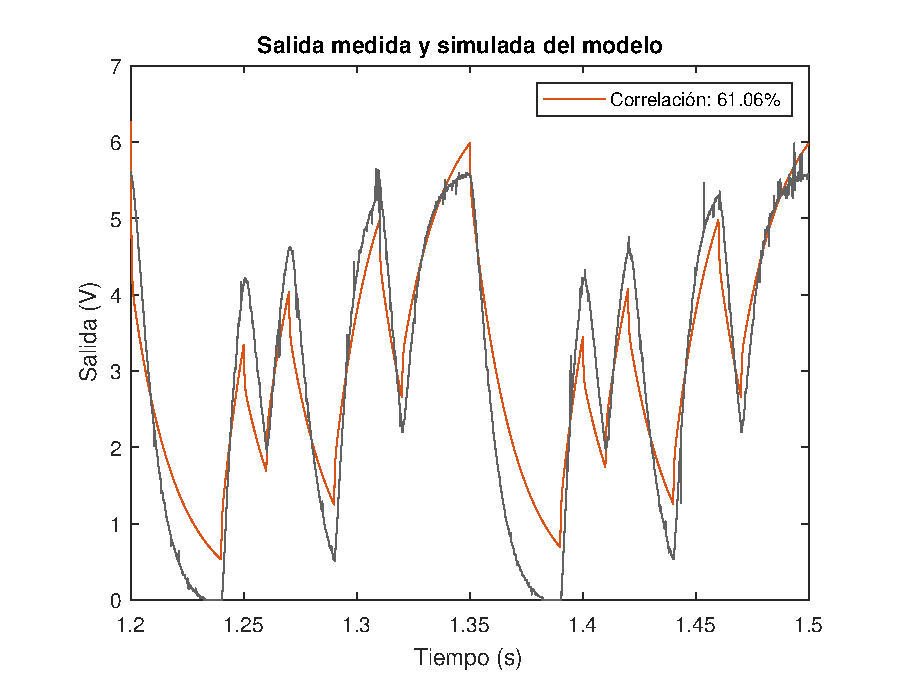
\includegraphics[width=10cm]{identificacion_comparacion.eps}
        %\vspace{-0.25cm}
        \caption{Comparación del modelo estimado con la respuesta medida.}
        \vspace{0.25cm}
        \label{fig:identificacion_comparacion}
    \end{subfigure}
    \begin{subfigure}[b]{\textwidth}
        \centering
        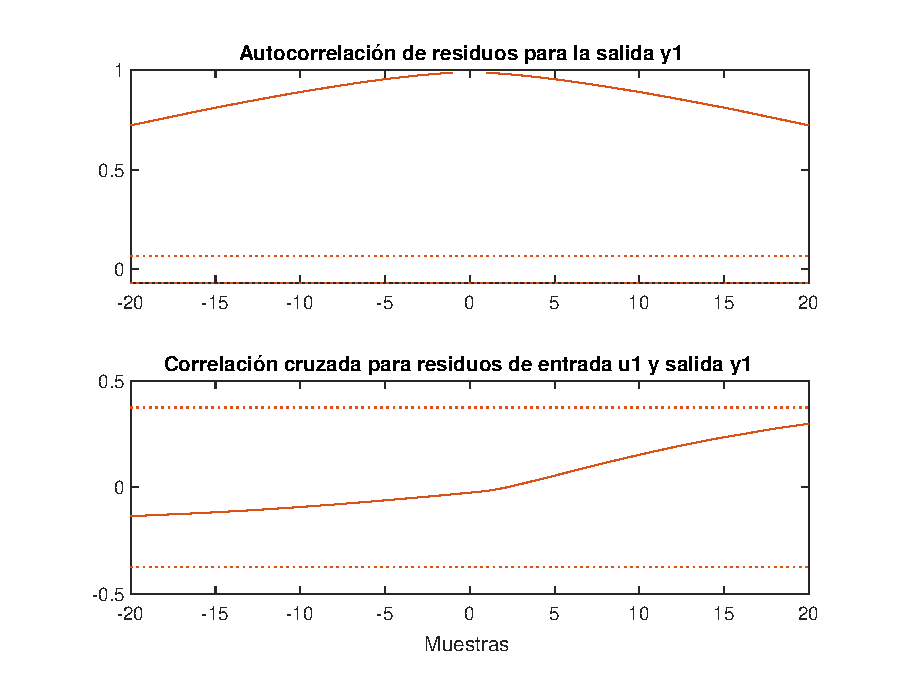
\includegraphics[width=10cm]{identificacion_residuos.eps}
        %\vspace{-0.25cm}
        \caption{Análisis residual del modelo estimado.}
        \label{fig:identificacion_residuos}
    \end{subfigure}

    \vspace{-0.25cm}
    \caption{Resultados de la estimación del modelo del sistema.}
    \label{fig:identificacion_resultados}
\end{figure}
\vspace{-0.5cm}

Como se puede observar en la Figura \ref{fig:identificacion_comparacion}, el modelo estimado coincide
con la respuesta medida del sistema (señal de validación) en un 61.06\%. El análisis residual del modelo estimado
no demuestra un buen resultado en la autocorrelación de residuales para la salida, pero sí demuestra un buen resultado 
para la correlación cruzada de residuales entre la entrada y la salida. Si bien se puede obtener un modelo
con mayor correlación con la salida medida y con un mejor resultado de análisis residual agregando un factor
de perturbación $K$, este modelo presenta mejores resultados en la práctica.

El modelo continuo estimado en espacios de estado es el siguiente:

\vspace{-0.5cm}
\begin{equation}
    \begin{cases}
        \begin{bmatrix}
            \dot{x_1}   \\
            \dot{x_2}   
        \end{bmatrix}
        =

        \begin{bmatrix}
            0   &   1 \\
            -1.914 \times 10^5   &  -3744           
        \end{bmatrix}

        \cdot
        \begin{bmatrix}
            x_1 \\
            x_2 
        \end{bmatrix}
        +
        \begin{bmatrix}
            2.214 \\
            -7000           
        \end{bmatrix}
        \cdot
        u 
        \\
        \\
        y =
        \begin{bmatrix}
            1 & 0
        \end{bmatrix}
        \cdot
        \begin{bmatrix}
            x_1 \\
            x_2
        \end{bmatrix}

    \end{cases}
    \label{eq:modelo_continuo}
\end{equation}
\vspace{-0.5cm}

Discretizando mediante retención de orden cero (zoh), con un tiempo de muestreo de $0.001\ s$, se obtiene:

\vspace{-0.5cm}
\begin{equation}
    \begin{cases}
        \begin{bmatrix}
            \dot{x_1}   \\
            \dot{x_2}   
        \end{bmatrix}
        =

        \begin{bmatrix}
            0.9626   &   0.000254 \\
            -48.61   &  0.01175           
        \end{bmatrix}

        \cdot
        \begin{bmatrix}
            x_1 \\
            x_2 
        \end{bmatrix}
        +
        \begin{bmatrix}
            0.0008139 \\
            -1.861           
        \end{bmatrix}
        \cdot
        u 
        \\
        \\
        y =
        \begin{bmatrix}
            1 & 0
        \end{bmatrix}
        \cdot
        \begin{bmatrix}
            x_1 \\
            x_2
        \end{bmatrix}

    \end{cases}
    \label{eq:modelo_discreto}
\end{equation}
\vspace{-0.5cm}

El mismo se puede representar en función de transferencia luego de transformarlo mediante MATLAB:   

\vspace{-0.5cm}
\begin{equation}
    H(z) = \dfrac{0.0008138\ z^{-1} - 0.0004821\ z^{-2}}{1 - 0.9744\ z^{-1} + 0.02366\ z^{-2}}
\end{equation}
\vspace{-0.5cm}

A continuación se grafican las respuestas temporal y en frecuencia del sistema identificado:

\begin{figure}[H]
    \centering

    \begin{subfigure}[b]{0.49\textwidth}
        \centering
        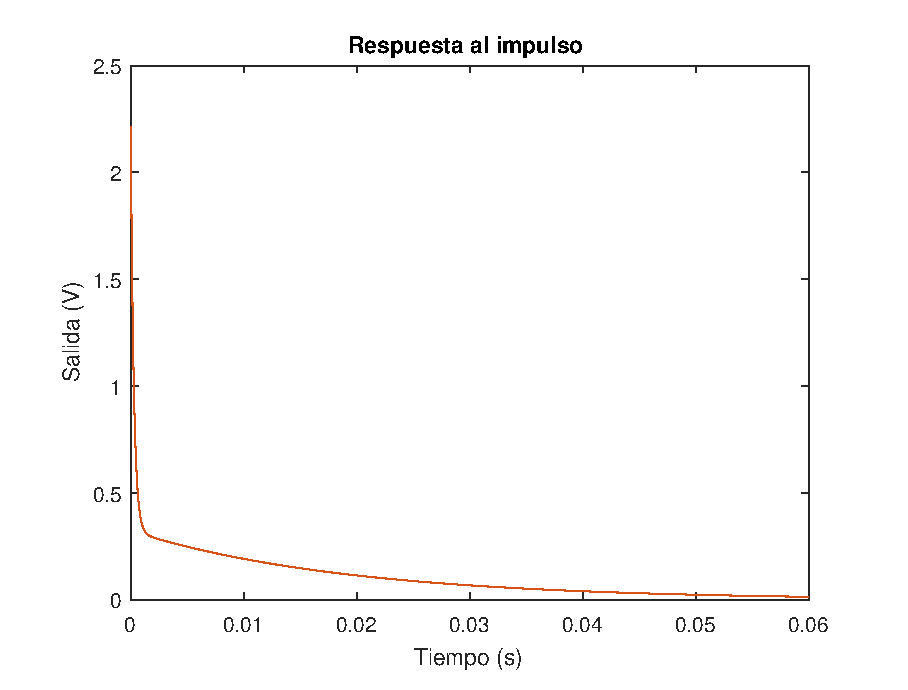
\includegraphics[width=\textwidth]{estimado_impulse.eps}
        %\vspace{-0.25cm}
        \caption{Respuesta al impulso.}
        \label{fig:estimado_impulse}
    \end{subfigure}
    \begin{subfigure}[b]{0.49\textwidth}
        \centering
        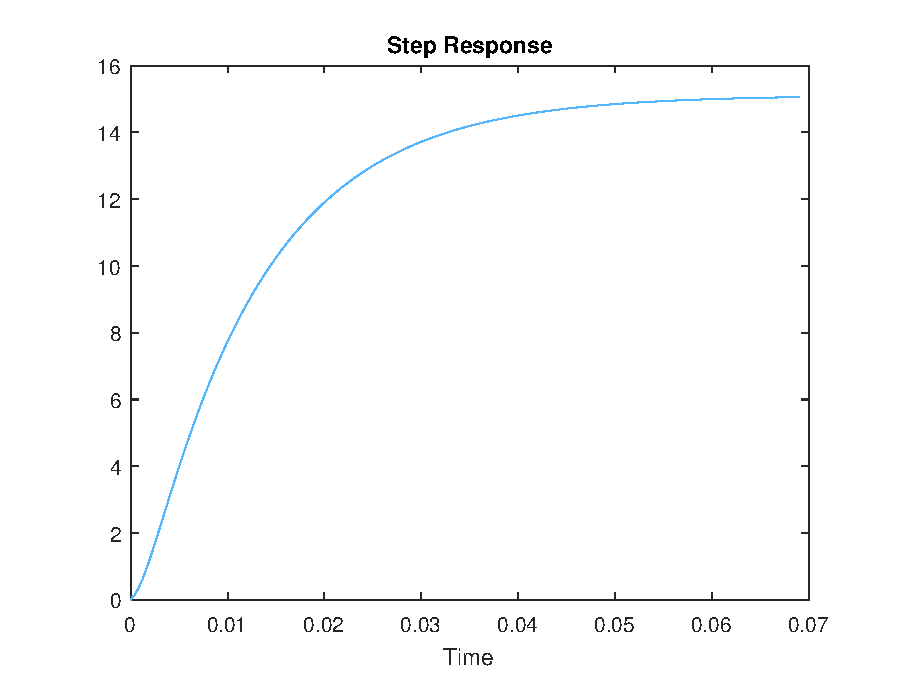
\includegraphics[width=\textwidth]{estimado_step.eps}
        %\vspace{-0.25cm}
        \caption{Respuesta al escalón.}
        \label{fig:estimado_step}
    \end{subfigure}

    \vspace{-0.25cm}
    \caption{Respuesta temporal del sistema estimado.}
    \label{fig:estimado_temporal}
\end{figure}
\vspace{-0.5cm}

\begin{figure}[H]
    \centering

    \begin{subfigure}[b]{0.49\textwidth}
        \centering
        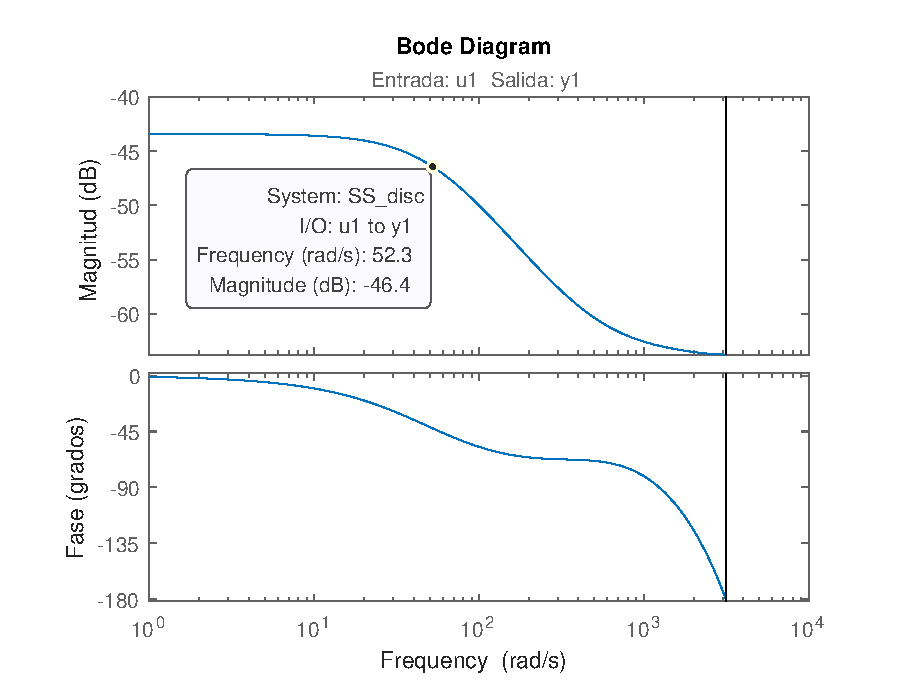
\includegraphics[width=\textwidth]{estimado_bode.eps}
        %\vspace{-0.25cm}
        \caption{Diagrama de Bode.}
        \label{fig:estimado_bode}
    \end{subfigure}
    \begin{subfigure}[b]{0.49\textwidth}
        \centering
        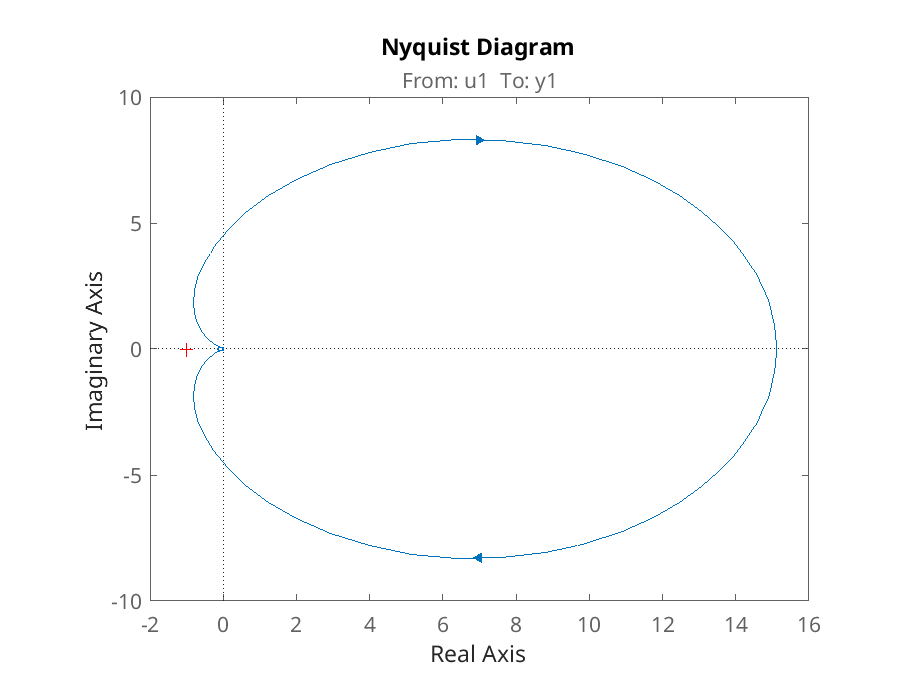
\includegraphics[width=\textwidth]{estimado_nyquist.eps}
        %\vspace{-0.25cm}
        \caption{Diagrama de Nyquist.}
        \label{fig:estimado_nyquist}
    \end{subfigure}

    \vspace{-0.25cm}
    \caption{Respuesta en frecuencia del sistema estimado.}
    \label{fig:estimado_frecuencia}
\end{figure}
\vspace{-0.5cm}

Como se puede observar en la figura \ref{fig:estimado_bode}, el sistema tiene una frecuencia de corte 
de $52.3\ rad/s$ (ya que la banda de paso es de $43.4\ dB$). Por lo tanto, el ancho de banda del sistema
identificado es de $8.32\ Hz$

\vspace{-0.5cm}
\subsection{\textbf{Análisis de estabilidad}}
\vspace{-0.5cm}

\begin{figure}[H]
    \centering

    \begin{subfigure}[b]{0.49\textwidth}
        \centering
        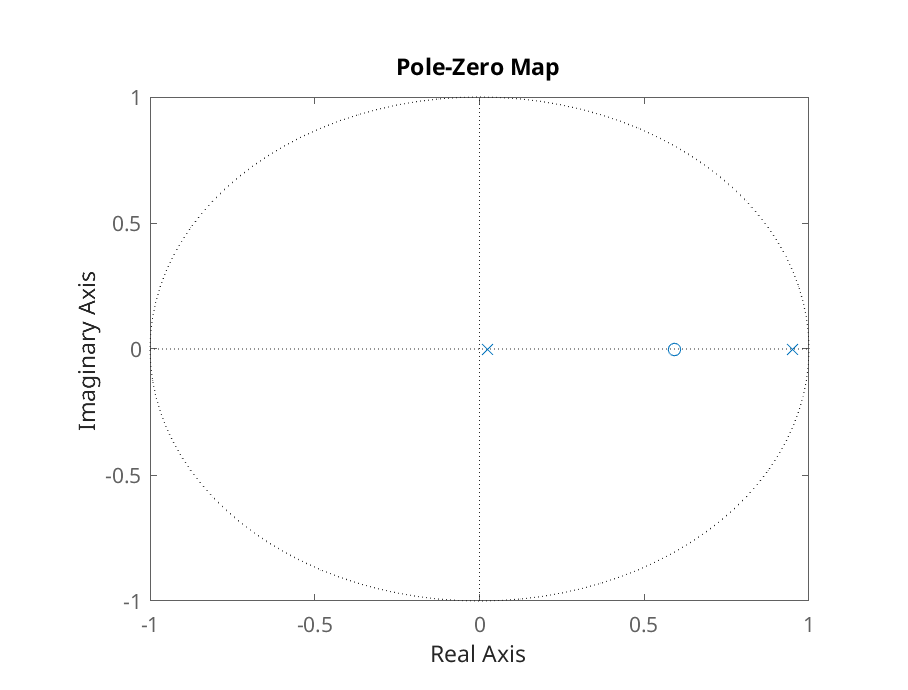
\includegraphics[width=\textwidth]{estimado_pzmap.eps}
        %\vspace{-0.25cm}
        \caption{Mapa de polos y ceros.}
        \label{fig:estimado_pzmap}
    \end{subfigure}
    \begin{subfigure}[b]{0.49\textwidth}
        \centering
        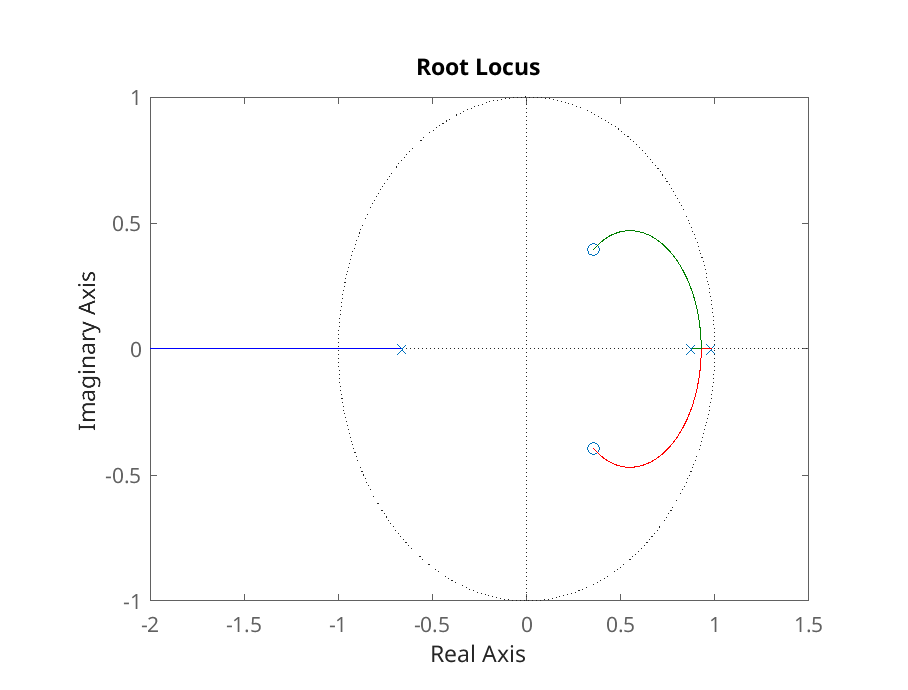
\includegraphics[width=\textwidth]{estimado_rlocus.eps}
        %\vspace{-0.25cm}
        \caption{Lugar geométrico de las raíces.}
        \label{fig:estimado_rlocus}
    \end{subfigure}

    \vspace{-0.25cm}
    \caption{Análisis de la respuesta temporal del sistema estimado.}
    \label{fig:estimado_estabilidad}
\end{figure}
\vspace{-0.5cm}

La respuesta al impulso del sistema converge a cero cuando el tiempo tiende al infinito.
En la respuesta al escalón, el sistema converge a un valor.
La ubicación de polos y el lugar geométricos de las raíces están ubicados dentro 
del círculo unitario en el plano z. Además, en la figura \ref{fig:estimado_nyquist}, la curva no rodea
el punto crítico (-1, 0). Debido a estas características se determina que el sistema es estable.

En la figura \ref{fig:estimado_rlocus}, se observa que para ciertos parámetros del sistema, un polo puede
ubicarse por fuera del círculo unitario en el plano z, resultando en un sistema inestable.

\vspace{-0.5cm}
\subsection{\textbf{Implementación en microcontrolador - PID}}
\vspace{-0.5cm}

Para implementar el sistema de control PID en el microcontrolador, se implementó un timer de 200 microsegundos,
que llama a una función de control cada vez que termina. Este temporizador corre periódicamente durante el funcionamiento
del programa. Se configura también un canal de PWM para controlar el MOSFET del convertidor buck, con frecuencia de 19 kHz
y ciclo de trabajo variable.

En la función de control, se mide el valor del ADC (convertidor analógico a digital) para obtener el
valor de setpoint, que varía de 0 V a 12 V. Luego, se mide por el ADC el valor de la retroalimentación, que, aplicada
a una curva de calibración, se obtiene el valor de tensión de salida. El setpoint restado a este valor resulta en
el error que, ingresado en la fórmula de ecuación en diferencias del controlador PID con filtro derivativo, se obtiene
la señal de control. Esta señal se aplica al PWM (modulación por ancho de pulso) del pin de salida que controla
el MOSFET del convertidor buck.

La programación se realizó mediante esp-idf, utilizando la referencia de API oficial de Espressif para el ESP32-S3. \parencite{ESPIDF}

\vspace{-0.5cm}
\subsection{\textbf{Resultados controlador PID}}
\vspace{-0.5cm}

A continuación se presentan distintas figuras con diferentes valores de constantes Kp, Ki, Kd y N. Se configura
un setpoint fijo de 6,00 V, a excepción de la figura \ref{fig:pid1}, que se configura un setpoint de 5,50 V.

\begin{figure}[H]
    \centering

    \begin{subfigure}[b]{0.49\textwidth}
        \centering
        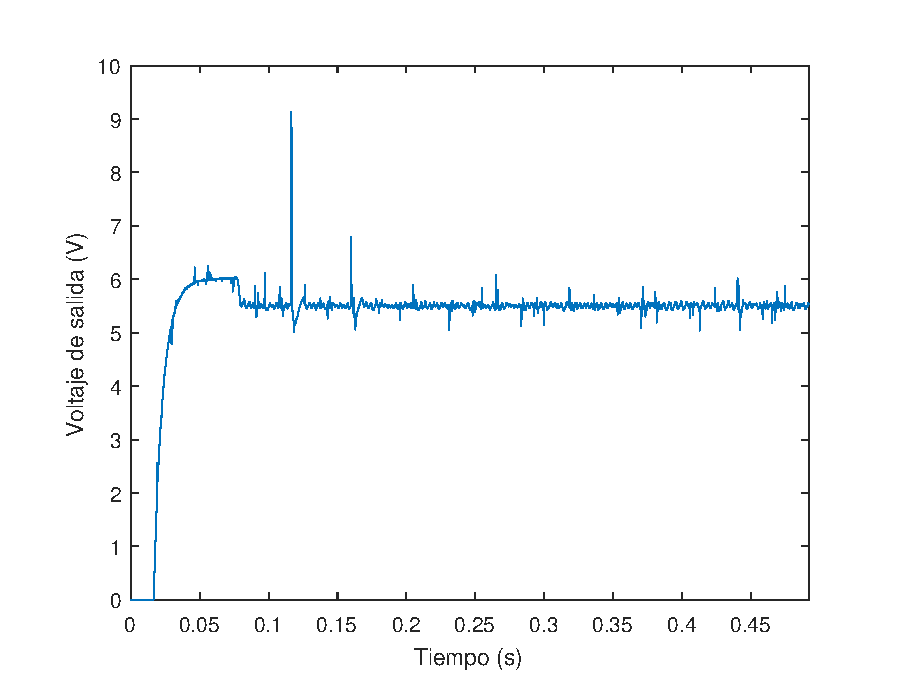
\includegraphics[width=\textwidth]{pid_1.eps}
        %\vspace{-0.25cm}
        \caption{Salida (V) según microcontrolador.}
        \label{fig:pid1_micro}
    \end{subfigure}
    \begin{subfigure}[b]{0.49\textwidth}
        \centering
        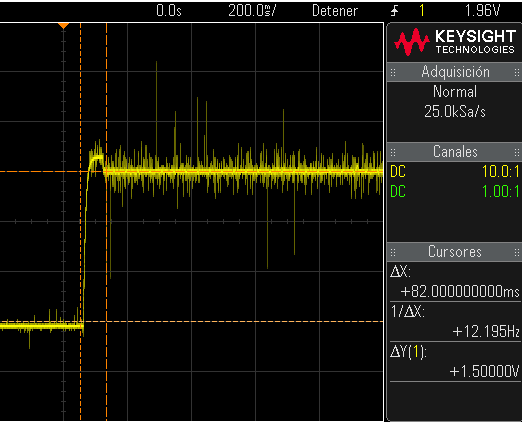
\includegraphics[width=\textwidth]{pid_1_osc.png}
        %\vspace{-0.25cm}
        \caption{Retroalimentación (V) según osciloscopio.}
        \label{fig:pid1_osciloscopio}
    \end{subfigure}

    \vspace{-0.25cm}
    \caption{Respuesta temporal con Kp=0,02; Ki=9,78; Kd=0; N=92,75.}
    \label{fig:pid1}
\end{figure}
\vspace{-0.5cm}

\begin{figure}[H]
    \centering

    \begin{subfigure}[b]{0.49\textwidth}
        \centering
        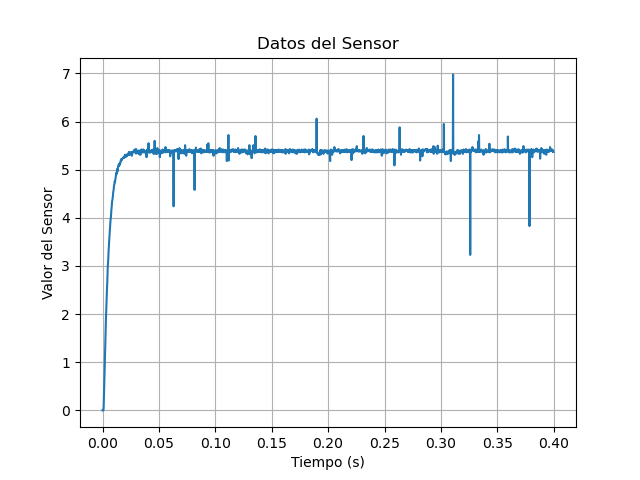
\includegraphics[width=\textwidth]{Kp0,5.png}
        %\vspace{-0.25cm}
        \caption{Señal de salida (Volts).}
        \label{fig:pid_solokp_salida}
    \end{subfigure}
    \begin{subfigure}[b]{0.49\textwidth}
        \centering
        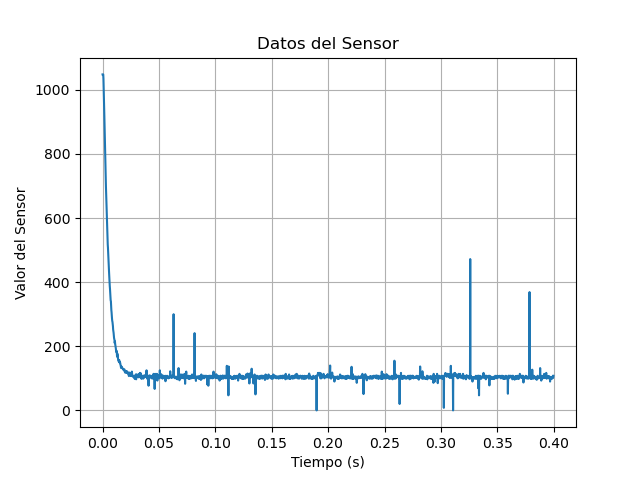
\includegraphics[width=\textwidth]{Kp0,5_c.png}
        %\vspace{-0.25cm}
        \caption{Señal de control (duty cycle en bits).}
        \label{fig:pid_solokp_control}
    \end{subfigure}

    \vspace{-0.25cm}
    \caption{Respuesta temporal con Kp=0,5; Ki=0; Kd=0; N=0.}
    \label{fig:pid_solokp}
\end{figure}
\vspace{-0.5cm}

Como se aprecia en la figura \ref{fig:pid_solokp} observa un error de estado estacionario debido a que se configura un control
solamente proporcional.

\begin{figure}[H]
    \centering

    \begin{subfigure}[b]{0.49\textwidth}
        \centering
        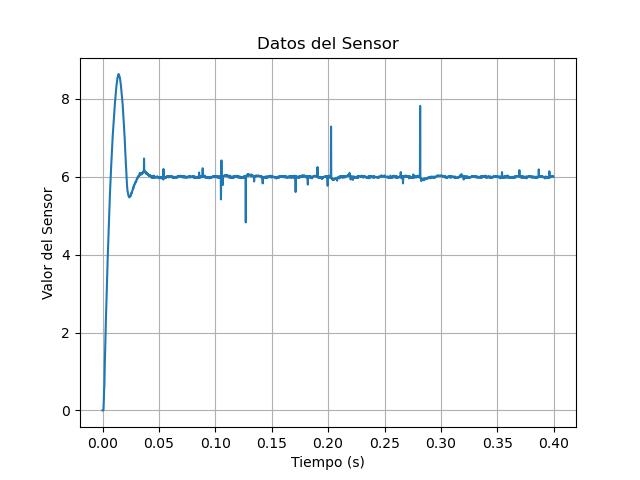
\includegraphics[width=\textwidth]{Kp1Ki500Kd0N0.png}
        %\vspace{-0.25cm}
        \caption{Señal de salida (Volts).}
        \label{fig:pid_kialto_salida}
    \end{subfigure}
    \begin{subfigure}[b]{0.49\textwidth}
        \centering
        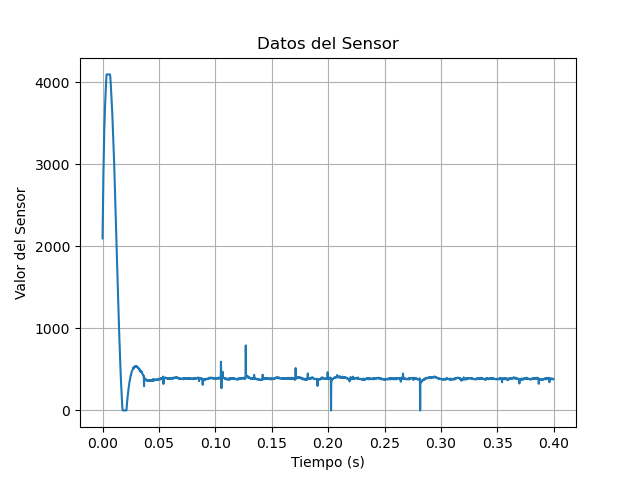
\includegraphics[width=\textwidth]{Kp1Ki500Kd0N0_c.png}
        %\vspace{-0.25cm}
        \caption{Señal de control (duty cycle en bits).}
        \label{fig:pid_kialto_control}
    \end{subfigure}

    \vspace{-0.25cm}
    \caption{Respuesta temporal con Kp=1; Ki=500; Kd=0; N=0.}
    \label{fig:pid_kialto}
\end{figure}
\vspace{-0.5cm}

\begin{figure}[H]
    \centering

    \begin{subfigure}[b]{0.49\textwidth}
        \centering
        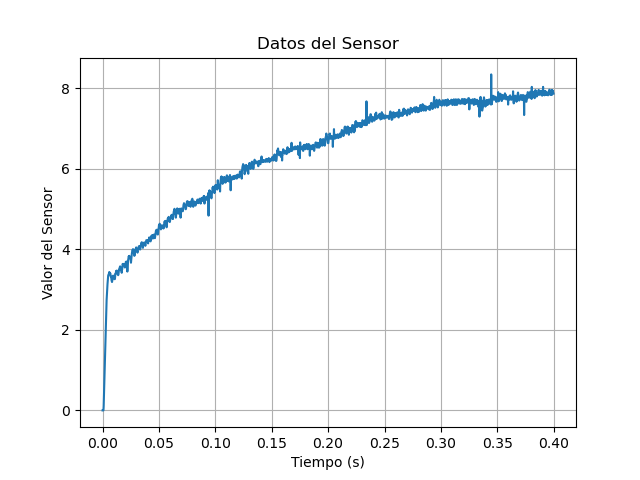
\includegraphics[width=\textwidth]{Kp1Ki0Kd5N500.png}
        %\vspace{-0.25cm}
        \caption{Señal de salida (Volts).}
        \label{fig:pid_kdalto_salida}
    \end{subfigure}
    \begin{subfigure}[b]{0.49\textwidth}
        \centering
        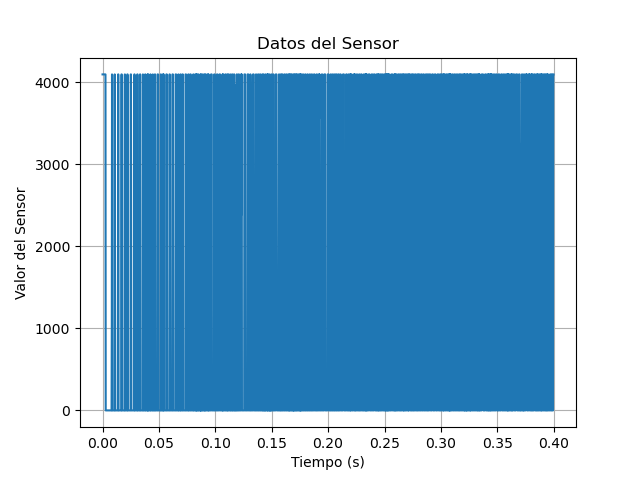
\includegraphics[width=\textwidth]{Kp1Ki0Kd5N500_c.png}
        %\vspace{-0.25cm}
        \caption{Señal de control (duty cycle en bits).}
        \label{fig:pid_kdalto_control}
    \end{subfigure}

    \vspace{-0.25cm}
    \caption{Respuesta temporal con Kp=1; Ki=0; Kd=5; N=500.\protect \footnotemark}
    \label{fig:pid_kdalto}
\end{figure}
\vspace{-0.5cm}

\footnotetext{Una constante derivativa alta inestabiliza el sistema.}

Finalmente se decide utilizar la siguiente configuración de control PID:

\begin{figure}[H]
    \centering

    \begin{subfigure}[b]{0.49\textwidth}
        \centering
        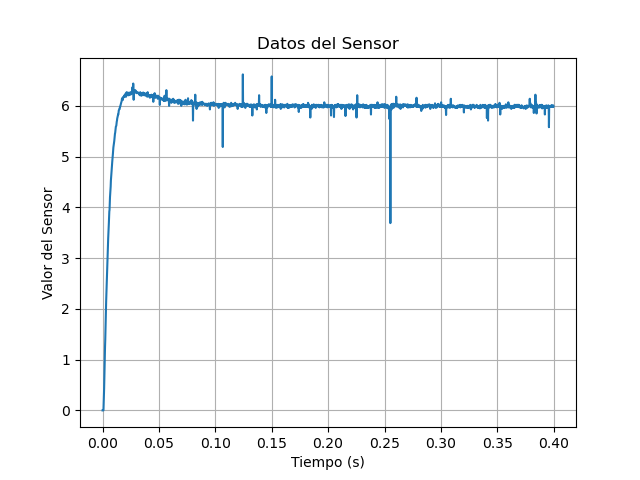
\includegraphics[width=\textwidth]{Kp0,5381Ki52,39Kd0,0002741N543,18.png}
        %\vspace{-0.25cm}
        \caption{Señal de salida (Volts).}
        \label{fig:pid_final_salida}
    \end{subfigure}
    \begin{subfigure}[b]{0.49\textwidth}
        \centering
        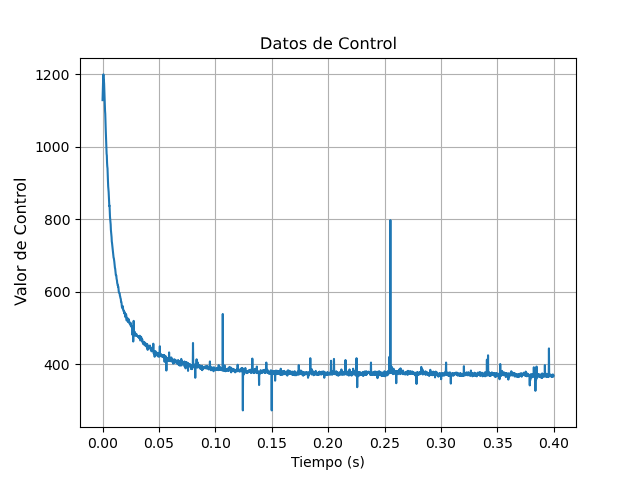
\includegraphics[width=\textwidth]{Kp0,5381Ki52,39Kd0,0002741N543,18_c.png}
        %\vspace{-0.25cm}
        \caption{Señal de control (duty cycle en bits).}
        \label{fig:pid_final_control}
    \end{subfigure}

    \vspace{-0.25cm}
    \caption{Respuesta temporal con Kp=0,54; Ki=52,39; Kd=2,74 $\times 10^{-4}$; N=543.}
    \label{fig:pid_final}
\end{figure}
\vspace{-0.5cm}

\vspace{-0.5cm}
\subsection{\textbf{Control en espacio de estados}}
\vspace{-0.5cm}

Antes de comenzar el desarrollo de un sistema de control en espacio de estados, se debe analizar
que el sistema cumpla con la condición para garantizar una controlabilidad completa. Para ello,
se calcula la matriz de controlabilidad, la cual debe ser de rango 2 (para un sistema de segundo orden).

\vspace{-0.5cm}
\begin{equation}
    Co
    =
    \begin{bmatrix}
        \textbf{B} & \textbf{AB}
    \end{bmatrix}
    =
    \begin{bmatrix}
        0.0008  & 0.0003    \\
        -1.8606 & -0.0614
    \end{bmatrix}
    \rightarrow
    \
    rank(Co) = 2\            
    \
    \therefore
    \ Sistema\  controlable
\end{equation}
\vspace{-0.5cm}

Observando la ecuación \ref{eq:modelo_continuo}, se tiene que la salida del sistema es igual
al estado $x_1$. Debido a que el sistema fue obtenido mediante el System Identification Toolbox de MATLAB,
el estado $x_2$ es desconocido, y para poder realizar un control es necesario obtener el valor del 
estado en cada momento. Por lo tanto, es necesario implementar algún tipo de observador.

Primero, se analiza si el sistema cumple con la condición para ser completamente observable:

\vspace{-0.5cm}
\begin{equation}
    Ob
    =
    \begin{bmatrix}
        \textbf{C}  \\ \textbf{CA}
    \end{bmatrix}
    =
    \begin{bmatrix}
        1.0000  &    0      \\ 
        0.9626  &    0.0003
    \end{bmatrix}
    \rightarrow
    \
    rank(Ob) = 2\            
    \
    \therefore
    \ Sistema\  completamente \ observable
\end{equation}
\vspace{-0.5cm}         

Como el sistema es controlable y completamente observable, se procede a diseñar un servosistema para que la
salida del sistema siga una referencia. En espacio de estados, se calcula una matriz de retroalimentación de estados
K que, aplicada en el sistema en espacio de estados, permite calcular una señal de control u para minimizar el error.
Sin embargo, si la planta no posee naturalmente un integrador, se debe insertar un integrador
en el camino directo entre el comparador de error y la planta, obteniendo el siguiente sistema:

\begin{figure}[H]
    \centering
    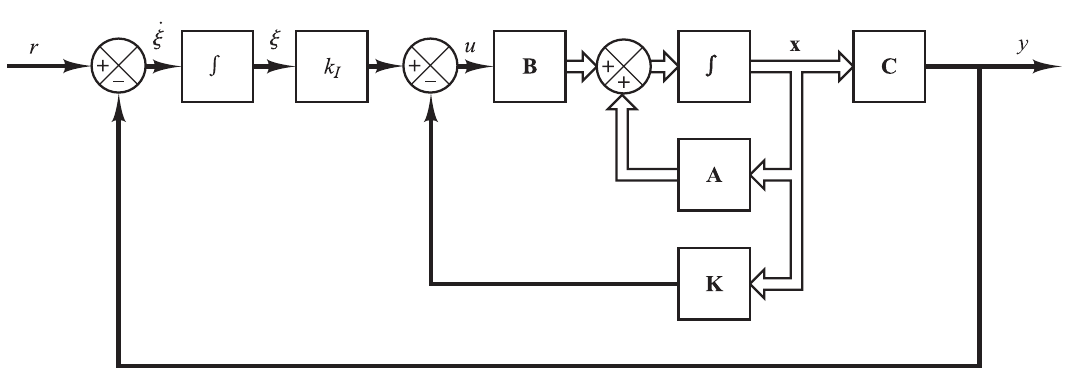
\includegraphics[height=5cm]{servo_diagrama.png}
    \vspace{-0.25cm}
    \caption{Servosistema de tipo 1.}
    \label{fig:servo_diagrama}
\end{figure}
\vspace{-0.5cm}

Donde:

\begin{itemize}[noitemsep]
    \item $\textbf{x} =$ vector de estado de la planta (vector de dimensión n estados).
    \item $\xi =$ salida del integrador.
    \item $r =$ señal de entrada de referencia.
    \item $\textbf{A}$ matriz de coeficientes constantes de $n\ x\ n$.
    \item $\textbf{B}$ matriz de coeficientes constantes de $n\ x\ 1$.
    \item $\textbf{C}$ matriz de coeficientes constantes de $1\ x\ n$.
\end{itemize}

Del diagrama, se pueden deducir las siguientes ecuaciones:

\vspace{-0.5cm}
\begin{equation}
    \begin{cases}
        \dot{\xi = r - y}
        \\
        u = -\textbf{K} \textbf{x} + k_i \xi
        \\
        \dot{\xi} = r - y = r - \textbf{C} \textbf{x}
    \end{cases}
\end{equation}

La dinámica del sistema se describe de la siguiente forma:

\vspace{-0.5cm}
\begin{equation}
        \begin{bmatrix}
            \dot{\textbf{x}}(t) \\
            \dot{\xi}(t)
        \end{bmatrix}
        =
        \begin{bmatrix}
            \textbf{A} & \textbf{0} \\
            -\textbf{C} & 0
        \end{bmatrix}
        \begin{bmatrix}
            \textbf{x}(t) \\
            \xi(t)
        \end{bmatrix}
        +
        \begin{bmatrix}
            \textbf{B} \\
            0
        \end{bmatrix}
        u(t)
        +
        \begin{bmatrix}
            \textbf{0} \\
            1
        \end{bmatrix}
        r(t)
    \label{eq:servosistema}
\end{equation}

Si se diseña un sistema asintóticamente estable, tal que los estados, el error y la entrada tiendan a valores constantes,
se obtiene:

\vspace{-0.5cm}
\begin{equation}
        \begin{bmatrix}
            \dot{\textbf{x}}_e(t) \\
            \dot{\xi}_e(t)
        \end{bmatrix}
        =
        \begin{bmatrix}
            \textbf{A} & \textbf{0} \\
            -\textbf{C} & 0
        \end{bmatrix}
        \begin{bmatrix}
            \dot{\textbf{x}}_e(t) \\
            \xi_e(t)
        \end{bmatrix}
        +
        \begin{bmatrix}
            \textbf{B} \\
            0
        \end{bmatrix}
        u_e(t)
\end{equation}

\vspace{-0.5cm}
\begin{equation}
    u_e(t) = -\textbf{K} \textbf{x}_e(t) + k_i \xi_e(t)
\end{equation}

Definiendo el vector de error e(t):

\vspace{-0.5cm}
\begin{equation}
    \textbf{e}(t) = \begin{bmatrix}
        \textbf{x}_e(t) \\
        \xi_e(t)
    \end{bmatrix}
\end{equation}

Se puede simplificar de la siguiente forma:

\vspace{-0.5cm}
\begin{equation}
    \dot{\textbf{e}} = \mathbf{\hat{A}} e + \mathbf{\hat{B}} u_e
    \label{eq:servo_error_Keue}
\end{equation}

\vspace{-0.5cm}

\begin{equation}
    u_e = -\mathbf{\hat{K}e}
    \label{eq:servo_error_Ke}
\end{equation}

Donde:

\vspace{-0.5cm}
\begin{equation}
    \mathbf{\hat{A}} = \begin{bmatrix}
        \textbf{A} & \textbf{0} \\
        -\textbf{C} & 0
    \end{bmatrix}
    , \quad
    \mathbf{\hat{B}} = \begin{bmatrix}
        \textbf{B} \\
        0
    \end{bmatrix}
    , \quad
    \mathbf{\hat{K}} = \begin{bmatrix}
        \textbf{K} & -k_i
    \end{bmatrix}
\end{equation}

Por lo tanto, se puede diseñar un sistema de control en espacio de estados solamente obteniendo valores
para la matriz de retroalimentación de estados $\mathbf{\hat{K}}$, que no solo contiene la matriz \textbf{K}
para los estados del sistema, sino también la constante de integración $k_i$.

Existen distintas técnicas para diseñar servosistemas mediante realimentación de estados: el método de asignación de polos,
el regulador lineal cuadrático (LQR), entre otros.

\textbf{Método de asignación de polos:} este método consiste, como dice su nombre, en asignar polos en lazo cerrado deseados para el sistema.
En un servosistema de tipo 1 como el que se desarrolló, se obtiene la ecuación de estado de error sustituyendo
la ecuación \ref{eq:servo_error_Ke} en la ecuación \ref{eq:servo_error_Keue}:

\vspace{-0.5cm}
\begin{equation}
    \dot{\textbf{e}} = (\mathbf{\hat{A}} - \mathbf{\hat{B}} \mathbf{\hat{K}}) e
\end{equation}

Se calcula entonces un valor de matriz de retroalimentación de estados $\mathbf{\hat{K}}$ que haga que los autovalores
de la matriz $(\mathbf{\hat{A}} - \mathbf{\hat{B}} \mathbf{\hat{K}})$ sean los polos deseados. Para ello, se utiliza la función
\textit{place} de MATLAB, que devuelve una matriz de ganancia $\mathit{K}$ de manera que el feedback de estado $\mathit{u = -Kx}$ ubique los polos
de lazo cerrado en las ubicaciones deseadas.\parencite{MATLAB_place}

El método de asignación de polos, aunque efectivo para garantizar la estabilidad y las especificaciones dinámicas deseadas del sistema, presenta una
desventaja considerable: la dificultad de determinar la ubicación óptima de los polos. A menudo, la selección de los polos depende de la experiencia
del diseñador y no siempre resulta evidente cuál es la configuración que garantizará el mejor compromiso entre rapidez de respuesta, amortiguamiento
y robustez.\parencite{OGATA} Por esa razón, se opta por utilizar el método siguiente:

\textbf{Regulador lineal cuadrático (LQR):} el regulador lineal cuadrático (LQR) es un método de control óptimo que, dada la ecuación del sistema:

\vspace{-0.5cm}
\begin{equation}
    \dot{\textbf{x}} = \textbf{A} \textbf{x} + \textbf{B} \textbf{u}
\end{equation}

determina la matriz de ganancia de realimentación de estados $\textbf{K}$:

\vspace{-0.5cm}
\begin{equation}
   \textbf{u}(t) = -\textbf{K} \textbf{x}(t)
\end{equation}

con el objetivo de minimizar la función de costo cuadrática:

\vspace{-0.5cm}
\begin{equation}
    J = \int_{0}^{\infty} (\textbf{x}^T \textbf{Q} \textbf{x} + \textbf{u}^T \textbf{R} \textbf{u}) dt
    \label{eq:costo_lqr}
\end{equation}

donde $\textbf{Q}$ es la matriz ponderada de coste de estado y $\textbf{R}$ es la matriz ponderada de coste de entrada.

Como la función de costo en la ecuación \ref{eq:costo_lqr} es cuadrática, existe una solución analítica para 
la óptima matriz de ganancia $\textbf{K}_r$ dada por:

\vspace{-0.5cm}
\begin{equation}
    \textbf{K}_r = \textbf{R}^{-1} \textbf{B}^T \textbf{X}
\end{equation}

donde $\textbf{X}$ es la solución de la ecuación de Riccati:

\vspace{-0.5cm}
\begin{equation}
    \textbf{A}^T \textbf{X} + \textbf{X} \textbf{A} - \textbf{X} \textbf{B} \textbf{R}^{-1} \textbf{B}^T \textbf{X} + \textbf{Q} = 0
    \label{eq:riccati}
\end{equation}

Resolviendo la ecuación \ref{eq:riccati} es numéricamente robusto y ya está implementado en varios lenguajes de programación.
En MATLAB, se utiliza la función \textit{lqr} para obtener la matriz de ganancia $\textbf{K}_r$.\parencite{MATLAB_lqr}

Seleccionar la mejor matriz de ganancias K para estabilizar el sistema sin gastar demasiado esfuerzo de control es un objetivo importante en el control óptimo.
Se debe encontrar un equilibrio entre la estabilidad del sistema en lazo cerrado y la agresividad del control.
Es fundamental tener en cuenta el gasto de control para: 1) evitar que el controlador reaccione de manera excesiva 
rente a ruidos y perturbaciones de alta frecuencia, 2) garantizar que la actuación no exceda las amplitudes máximas
permitidas, y 3) evitar que el control sea prohibitivamente costoso. \parencite{BRUNTON}

Para el sistema regulador del convertidor buck, se utiliza el modelo discreto obtenido en la ecuación \ref{eq:modelo_discreto},
se expande para incluir el integrador del servosistema tipo 1 de la ecuación \ref{eq:servosistema} y se calcula la matriz de 
realimentación de estados óptima $\mathbf{K}$ y la constante integradora $k_i$ mediante la función \textit{lqr} de MATLAB. Las matrices ponderadas
de coste son las siguientes:

\vspace{-0.5cm}
\begin{equation}
    Q =
    \begin{bmatrix}
        10000 & 0 & 0 \\
        0 & 10 & 0 \\
        0 & 0 & 10000
    \end{bmatrix}
    , \quad
    R = 0.1
\end{equation}

Se pondera la variable de estado $x_1$ con un valor de 10000, ya que es la variable de estado más importante para el sistema. El tercer
estado referencia la acción integral, por lo que se pondera con un valor alto. La variable de estado $x_2$ se pondera con un valor de 10,
ya que es la variable de estado menos importante para el sistema. La matriz de coste de entrada $R$ se pondera con un valor de 0.1, que
en la práctica resulta en una respuesta adecuada.

A continuación se presentan los resultados simulados:

\begin{figure}[H]
    \centering

    \begin{subfigure}[b]{0.49\textwidth}
        \centering
        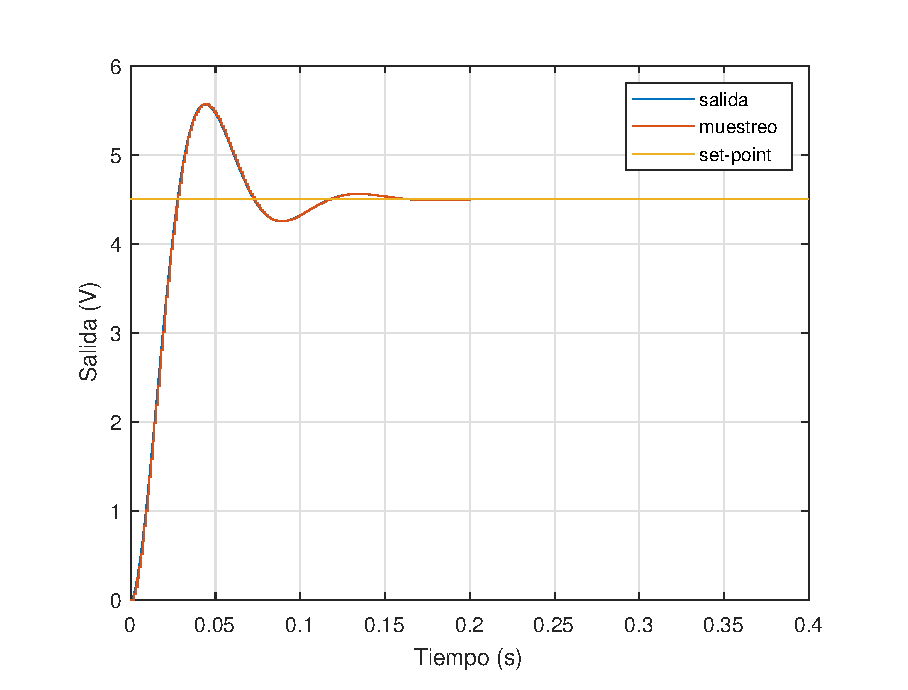
\includegraphics[width=\textwidth]{lqr_salida.eps}
        %\vspace{-0.25cm}
        \caption{Señal de salida (Volts).}
        \label{fig:lqr_simulacion_y}
    \end{subfigure}
    \begin{subfigure}[b]{0.49\textwidth}
        \centering
        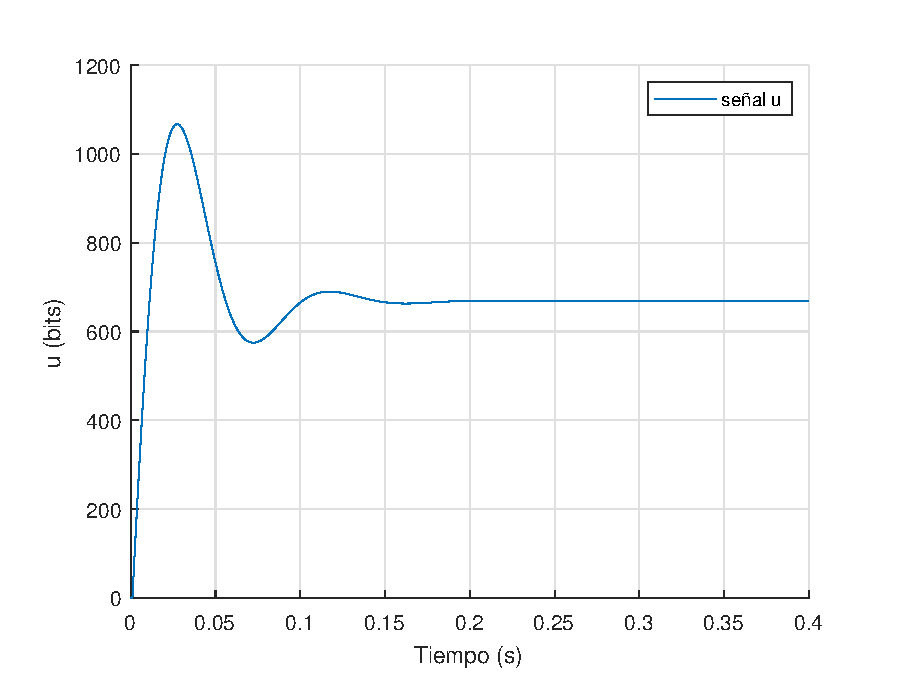
\includegraphics[width=\textwidth]{lqr_u.eps}
        %\vspace{-0.25cm}
        \caption{Señal de control (duty cycle en bits).}
        \label{fig:lqr_simulacion_u}
    \end{subfigure}

    \vspace{-0.25cm}
    \caption{Resultados de simulación de LQR.}
    \label{fig:lqr_simulacion}
\end{figure}
\vspace{-0.5cm}

\vspace{-0.25cm}
\subsubsection{\textbf{Diseño de observador}}
\vspace{-0.25cm}

Como se mencionó anteriormente, no se tiene acceso directo al estado $x_2$ del sistema, por lo que se debe diseñar un observador.
Existen distintos tipos de observadores, como el observador de Luenberger, el filtro de Kalman, entre otros. Un observador de estado 
estima las variables de estado basándose en las mediciones de las variables de salida y de control. Pueden diseñarse si y sólo si
se satisface la condición de observabilidad, que ya se demostró que se cumple en el sistema.

\textbf{Observador de Luenberger:} El observador de Luenberger es un subsistema para reconstruir el vector de estado de la planta.
El modelo matemático del observador es básicamente el mismo que el de la planta, salvo que se incluye un término adicional
que contiene el error de estimación para compensar las imprecisiones en las matrices A y B y la falta del error inicial.
El error de estimación o error de observación es la diferencia entre la salida medida y la salida estimada.

\begin{figure}[H]
    \centering
    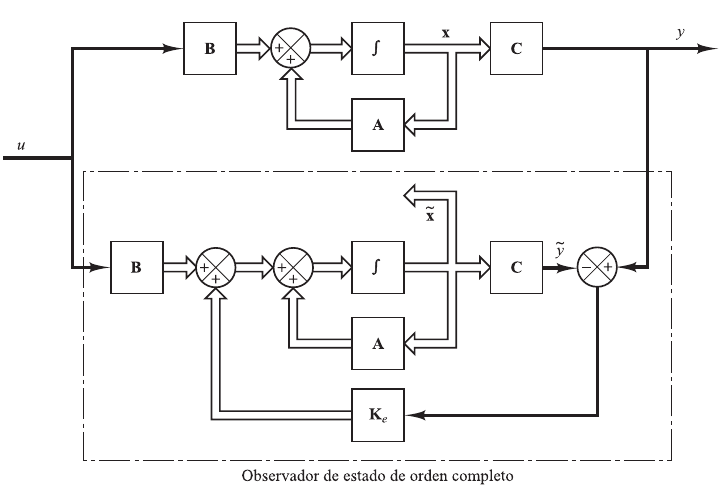
\includegraphics[height=8cm]{observador_diagrama.png}
    \vspace{-0.25cm}
    \caption{Diagrama de bloque del sistema y del observador de estado de orden completo}
    \label{fig:observador}
\end{figure}
\vspace{-0.5cm}

El modelo matemático del observador es el siguiente:

\vspace{-0.5cm}
\begin{equation}
    \mathbf{\dot{\tilde{x}}} = \textbf{A} \mathbf{\tilde{x}} + \textbf{B} u + \textbf{K}_e (y - \tilde{y})
    =
    \textbf{A} \mathbf{\tilde{x}} + \textbf{B} u + \textbf{K}_e (y - \textbf{C} \mathbf{\tilde{x}})
    =
    (\textbf{A} - \textbf{K}_e \textbf{C}) \mathbf{\tilde{x}} + \textbf{B} u + \textbf{K}_e y
\end{equation}
\vspace{-0.5cm}

La matriz $\textbf{K}_e$ se llama matriz de ganancia del observador, es una matriz de ponderación al término de corrección que involucra
la diferencia entre la salida medida y la salida estimada.

Ya que se implementará en un microcontrolador, se discretiza la ecuación para estimar el valor de un estado futuro utilizando
el valor actual de estados estimados, señal de control y medición de salida. La ecuación resultante es la siguiente:

\vspace{-0.5cm}
\begin{equation}
    \mathbf{\tilde{x}}(k+1) = (\textbf{A}_d - \textbf{K}_d \textbf{C}_d) \mathbf{\tilde{x}}(k) + \textbf{B}_d u(k) + \textbf{K}_e y(k)
\end{equation}

Trabajando las ecuaciones para obtener los estados estimados por separado, para utilizar en el microcontrolador, se obtiene:

\vspace{-0.5cm}
\begin{equation}
    \begin{bmatrix}
        \tilde{x}_1(k+1) \\
        \tilde{x}_2(k+1)
    \end{bmatrix}
    =
    \left(
        \begin{bmatrix}
            A_{11} & A_{12} \\
            A_{21} & A_{22}
        \end{bmatrix}
        -
        \begin{bmatrix}
            K_{e_{11}} \\
            K_{e_{21}}
        \end{bmatrix}
        \begin{bmatrix}
            C_{11} & C_{12}
        \end{bmatrix}    
    \right)
    \cdot
    \begin{bmatrix}
        \tilde{x}_1(k) \\
        \tilde{x}_2(k)
    \end{bmatrix}
    +
    \begin{bmatrix}
        B_{11} \\
        B_{21}
    \end{bmatrix}
    u(k)
    +
    \begin{bmatrix}
        K_{e_{11}} \\
        K_{e_{21}}
    \end{bmatrix}
    y(k)
\end{equation}
\vspace{-0.5cm}

\vspace{-0.5cm}
\begin{equation}
    \begin{bmatrix}
        \tilde{x}_1(k+1) \\
        \tilde{x}_2(k+1)
    \end{bmatrix}
    =
    \begin{bmatrix}
        (A_{11} - K_{e_{11}} C_{11}) \tilde{x}_1(k) + (A_{12} - K_{e_{11}} C_{12}) \tilde{x}_2(k)\\
        (A_{21} - K_{e_{21}} C_{11}) \tilde{x}_1(k) + (A_{22} - K_{e_{21}} C_{12}) \tilde{x}_2(k)
    \end{bmatrix}
    +
    \begin{bmatrix}
        B_{11} u(k)\\
        B_{21} u(k)
    \end{bmatrix}
    +
    \begin{bmatrix}
        K_{e_{11}} y(k)\\
        K_{e_{21}} y(k)
    \end{bmatrix}
\end{equation}
\vspace{-0.5cm}

\vspace{-0.5cm}
\begin{equation}
    \begin{cases}
        \tilde{x}_1(k+1) = (A_{11} - K_{e_{11}} C_{11}) \tilde{x}_1(k) + (A_{12} - K_{e_{11}} C_{12}) \tilde{x}_2(k) + B_{11} u(k) + K_{e_{11}} y(k)
        \\
        \tilde{x}_2(k+1) = (A_{21} - K_{e_{21}} C_{11}) \tilde{x}_1(k) + (A_{22} - K_{e_{21}} C_{12}) \tilde{x}_2(k) + B_{21} u(k) + K_{e_{21}} y(k)
    \end{cases}
\end{equation}
\vspace{-0.5cm}

Similar al método de asignación de polos para obtener la matriz de realimentación de estados $\textbf{K}$, aquí también se asignan polos para obtener
la matriz de ganancia del observador $\textbf{K}_e$, con la diferencia que la ecuación de estado de error ahora está dada por:

\vspace{-0.5cm}
\begin{equation}
    \dot{\textbf{e}} = (\mathbf{A} - \mathbf{K_e} \mathbf{C}) e + \mathbf{B} u
\end{equation}
\vspace{-0.5cm}

Por lo tanto, se calcula un valor de matriz de ganancia del observador $\mathbf{K}_e$ que haga que los autovalores de la matriz $(\mathbf{A} - \mathbf{K}_e \mathbf{C})$
sean los polos deseados.

Se realizaron pruebas con distintas configuraciones de polos para el observador en el convertidor, pero no se obtuvieron buenos resultados,
posiblemente debido al modelo identificado que no es exactamente igual al modelo real del sistema (en pruebas sobre un circuito con modelo
matemático obtenido, el observador funcionó a la perfección). Por lo tanto, se optó por no implementar este tipo de observador e intentar con otro.

\textbf{Filtro de Kalman:} El filtro de Kalman es un conjunto de ecuaciones matemáticas que proporciona un medio computacional eficiente (recursivo)
para estimar el estado de un proceso, de manera que minimiza el promedio del error cuadrático. El filtro es muy poderoso en varios aspectos:
permite estimaciones de estados pasados, presentes e incluso futuros, y puede hacerlo incluso cuando la naturaleza precisa del sistema 
modelado es desconocida.

El filtro de Kalman aborda el problema general de intentar estimar el estado \( x \in \mathbb{R}^n \) de un proceso controlado en tiempo discreto
que está gobernado por la ecuación diferencial estocástica lineal:

\vspace{-0.5cm}
\begin{equation}
    x_k = A x_{k-1} + B u_{k-1} + w_{k-1},
\end{equation}
\vspace{-0.5cm}

con una medición \( z \in \mathbb{R}^m \) que es:

\vspace{-0.5cm}
\begin{equation}
    z_k = H x_k + v_k.
\end{equation}
\vspace{-0.5cm}

Las variables aleatorias \( w_k \) y \( v_k \) representan el ruido del proceso y el ruido de medición (respectivamente). Se asume que son
independientes (entre sí), blancas y con distribuciones de probabilidad normales

\vspace{-0.5cm}
\begin{equation}
    p(w) \sim \mathcal{N}(0, Q),
\end{equation}
\vspace{-0.5cm}

\vspace{-0.5cm}
\begin{equation}
    p(v) \sim \mathcal{N}(0, R).
\end{equation}
\vspace{-0.5cm}

En la práctica, las matrices de covarianza del ruido del proceso \( Q \) y del ruido de medición \( R \) pueden cambiar en cada paso de tiempo
o medición, pero se asumen constantes. \parencite{WELCH}

El filtro de Kalman se basa en dos fases: la fase de predicción y la fase de actualización o corrección:

\textit{Fase de predicción:}
\begin{enumerate}
    \item Proyectar el estado siguiente:
    
    \vspace{-0.5cm}
    \begin{equation}
        \mathbf{\hat{x}_p} = \textbf{A} \mathbf{\hat{x}_{(k-1)}} + \textbf{B} u_{(k-1)}
    \end{equation}
    \vspace{-0.5cm}

    \item Proyectar la matriz de covarianza del error de estimación:
    
    \vspace{-0.5cm}
    \begin{equation}
        \mathbf{P_{k_p}} = \textbf{A} \mathbf{P_{k_{(k-1)}}} \textbf{A}^T + \textbf{Q}
    \end{equation}
    \vspace{-0.5cm}

\end{enumerate}

\textit{Fase de corrección:}
\begin{enumerate}
    \item Calcular la ganancia de Kalman:

    \vspace{-0.5cm}
    \begin{equation}
        \mathbf{K} = (\mathbf{P_{k_p}}\ \textbf{C}^T) \cdot ({\textbf{C}\ \mathbf{P_{k_p}}\ \textbf{C}^T + \textbf{R}})^{-1}
    \end{equation}
    \vspace{-0.5cm}

    \item Actualizar la estimación del estado:
    
    \vspace{-0.5cm}
    \begin{equation}
        \mathbf{\hat{x}_k} = \mathbf{\hat{x}_p} + \mathbf{K} (y - \hat{y})
    \end{equation}
    \vspace{-0.5cm}

    \item Actualizar la matriz de covarianza del error de estimación:
    
    \vspace{-0.5cm}
    \begin{equation}
        \mathbf{P_k} = (\textbf{I} - \mathbf{K} \mathbf{C}) \mathbf{P_{k_p}}
    \end{equation}
    \vspace{-0.5cm}
\end{enumerate}

Para la implementación del filtro en el microcontrolador, se procede a analizar las ecuaciones para calcular cada elemento
de cada matriz por separado:

\textit{Predicción de los estados siguientes:}

\vspace{-0.5cm}
\begin{equation}
    \begin{bmatrix}
        \hat{x}_{1_{pred}} \\
        \hat{x}_{2_{pred}} 
    \end{bmatrix}
    =
    \begin{bmatrix}
        a_{11} + a_{12} \\
        a_{21} + a_{22}
    \end{bmatrix}
    \begin{bmatrix}
        \hat{x}_{1}(k) \\
        \hat{x}_{2}(k)
    \end{bmatrix}
    +
    \begin{bmatrix}
        b_{11} \\
        b_{21}
    \end{bmatrix}
    u(k)
\end{equation}
\vspace{-0.5cm}

\vspace{-0.5cm}
\begin{equation}
    \begin{cases}
        \hat{x}_{1_{pred}} = a_{11} \hat{x}_{1}(k) + a_{12} \hat{x}_{2}(k) + b_{11} u(k)
        \\
        \hat{x}_{2_{pred}} = a_{21} \hat{x}_{1}(k) + a_{22} \hat{x}_{2}(k) + b_{21} u(k)
    \end{cases}
\end{equation}
\vspace{-0.5cm}

\textit{Predicción de la matriz de covarianza de error de estimación:}

\vspace{-0.5cm}
\begin{equation}
    \begin{bmatrix}
        P_{k_{p_{11}}} & P_{k_{p_{12}}} \\
        P_{k_{p_{21}}} & P_{k_{p_{22}}}
    \end{bmatrix}
    =
    \begin{bmatrix}
        a_{11} & a_{12} \\
        a_{21} & a_{22}
    \end{bmatrix}
    \cdot
    \begin{bmatrix}
        P_{k_{11}} & P_{k_{12}} \\
        P_{k_{21}} & P_{k_{22}}
    \end{bmatrix}
    \cdot
    \begin{bmatrix}
        a_{11} & a_{21} \\
        a_{12} & a_{22}
    \end{bmatrix}
    +
    \begin{bmatrix}
        q_{11} & 0 \\
        0 & q_{22}
    \end{bmatrix}
\end{equation}
\vspace{-0.5cm}

\vspace{-0.5cm}
\begin{equation}
    \begin{cases}
        P_{k_{p_{11}}} = (a_{11}P_{k_{11}} + a_{12}P_{k_{21}})\ a_{11} + (a_{11}a_{12}P_{k_{12}} + a_{12}a_{22}P_{k_{22}})\ a_{12} + q_{11}
        \\
        P_{k_{p_{12}}} = (a_{11}P_{k_{12}} + a_{12}P_{k_{22}})\ a_{11} + (a_{11}a_{12}P_{k_{12}} + a_{12}a_{22}P_{k_{22}})\ a_{12}
        \\
        P_{k_{p_{21}}} = (a_{21}P_{k_{11}} + a_{22}P_{k_{21}})\ a_{21} + (a_{21}a_{12}P_{k_{12}} + a_{22}a_{22}P_{k_{22}})\ a_{22}
        \\
        P_{k_{p_{22}}} = (a_{21}P_{k_{12}} + a_{22}P_{k_{22}})\ a_{21} + (a_{21}a_{12}P_{k_{12}} + a_{22}a_{22}P_{k_{22}})\ a_{22} + q_{22}
    \end{cases}
\end{equation}
\vspace{-0.5cm}

\textit{Cálculo de la ganancia de Kalman:}

\vspace{-0.5cm}
\begin{equation}
    \begin{bmatrix}
        K_{1} \\
        K_{2}
    \end{bmatrix}
    =
    \left(
    \begin{bmatrix}
        P_{k_{p_{11}}} + P_{k_{p_{12}}} \\
        P_{k_{p_{21}}} + P_{k_{p_{22}}}
    \end{bmatrix}
    \cdot
    \begin{bmatrix}
        c_{11} \\
        c_{12}
    \end{bmatrix}
    \right)
    \cdot
    \left(
    \begin{bmatrix}
        c_{11} && c_{12}
    \end{bmatrix}
    \cdot
    \begin{bmatrix}
        P_{k_{p_{11}}} & P_{k_{p_{12}}} \\
        P_{k_{p_{21}}} & P_{k_{p_{22}}}
    \end{bmatrix}
    \cdot
    \begin{bmatrix}
        c_{11} \\
        c_{12}
    \end{bmatrix}
    +
    R
    \right)^{-1}
\end{equation}
\vspace{-0.5cm}

\vspace{-0.5cm}
\begin{equation}
    \begin{cases}
        S = c_{11}\ (P_{k_{p_{11}}} + c_{12}\ P_{k_{p_{21}}}) + c_{12}\ (c_{11}\ P_{k_{p_{12}}} + c_{12}\ P_{k_{p_{22}}}) + R
        \\
        K_{11} = (P_{k_{p_{11}}}\ c_{11} + P_{k_{p_{12}}}\ c_{12}) \cdot S^{-1} 
        \\
        K_{21} = (P_{k_{p_{21}}}\ c_{11} + P_{k_{p_{22}}}\ c_{12}) \cdot S^{-1}
    \end{cases}
\end{equation}
\vspace{-0.5cm}

\textit{Salida estimada con los estados predichos}

\vspace{-0.5cm}
\begin{equation}
    \hat{y} =
    \begin{bmatrix}
        c_{11} & c_{12}
    \end{bmatrix}
    \cdot
    \begin{bmatrix}
        \hat{x}_{1_{pred}} \\
        \hat{x}_{2_{pred}}
    \end{bmatrix}
    =
    c_{11} \cdot \hat{x}_{1_{pred}} + c_{12} \cdot \hat{x}_{2_{pred}}
\end{equation}
\vspace{-0.5cm}

\textit{Corrección de estados}

\vspace{-0.5cm}
\begin{equation}
    \begin{bmatrix}
        \hat{x}_{1}(k) \\
        \hat{x}_{2}(k) 
    \end{bmatrix}
    =
    \begin{bmatrix}
        \hat{x}_{1_{pred}} \\
        \hat{x}_{2_{pred}}
    \end{bmatrix}
    +
    \begin{bmatrix}
        K_{11} \\
        K_{21}
    \end{bmatrix}
    \cdot
    (y(k) - \hat{y}(k))
\end{equation}
\vspace{-0.5cm}

\vspace{-0.5cm}
\begin{equation}
    \begin{cases}
        \hat{x}_{1}(k) = \hat{x}_{1_{pred}} + K_{11} \cdot (y(k) - \hat{y}(k))
        \\
        \hat{x}_{2}(k) = \hat{x}_{2_{pred}} + K_{21} \cdot (y(k) - \hat{y}(k))
    \end{cases}
\end{equation}
\vspace{-0.5cm}

\textit{Corrección de covarianza de error}

\vspace{-0.5cm}
\begin{equation}
    \begin{bmatrix}
        P_{k_{11}} & P_{k_{12}} \\
        P_{k_{21}} & P_{k_{22}}
    \end{bmatrix}
    =
    \left(
    \begin{bmatrix}
        1 & 0 \\
        0 & 1
    \end{bmatrix}
    -
    \begin{bmatrix}
        K_{11} \\
        K_{21}
    \end{bmatrix}
    \cdot
    \begin{bmatrix}
        c_{11} & c_{12}
    \end{bmatrix}
    \right)
    \cdot
    \begin{bmatrix}
        P_{k_{p_{11}}} & P_{k_{p_{12}}} \\
        P_{k_{p_{21}}} & P_{k_{p_{22}}}
    \end{bmatrix}
\end{equation}
\vspace{-0.5cm}

\vspace{-0.5cm}
\begin{equation}
    \begin{cases}
        P_{k_{11}} = (1 - K_{11} * c_{11}) * P_{k_{p_{11}}} - K_{11} * c_{12} * P_{k_{p_{21}}};
        \\
        P_{k_{12}} = (1 - K_{11} * c_{11}) * P_{k_{p_{12}}} - K_{11} * c_{12} * P_{k_{p_{22}}};
        \\
        P_{k_{21}} = (1 - K_{21} * c_{12}) * P_{k_{p_{21}}} - K_{21} * c_{11} * P_{k_{p_{11}}};
        \\
        P_{k_{22}} = (1 - K_{21} * c_{12}) * P_{k_{p_{22}}} - K_{21} * c_{11} * P_{k_{p_{12}}};
    \end{cases}
\end{equation}
\vspace{-0.5cm}

\vspace{-0.5cm}
\subsection{\textbf{Implementación en microcontrolador - LQR con integrador y filtro de Kalman}}
\vspace{-0.5cm}

Para la implementación del sistema regulador en espacio de estados, se realizaron algunas modificaciones.
Primero, se modificó el período del timer a 1000 microsegundos, para obtener una frecuencia de muestreo de 1 kHz.
Además, la frecuencia del pwm generado se redujo a 1 kHz, para evitar problemas de comportamiento no lineal del
transistor MOSFET.

Se procede a mostrar diferentes resultados con distintos valores de Q y R para el filtro de Kalman, utilizando
los valores de K y ki obtenidos anteriormente para el LQR:

\begin{figure}[H]
    \centering

    \begin{subfigure}[b]{0.49\textwidth}
        \centering
        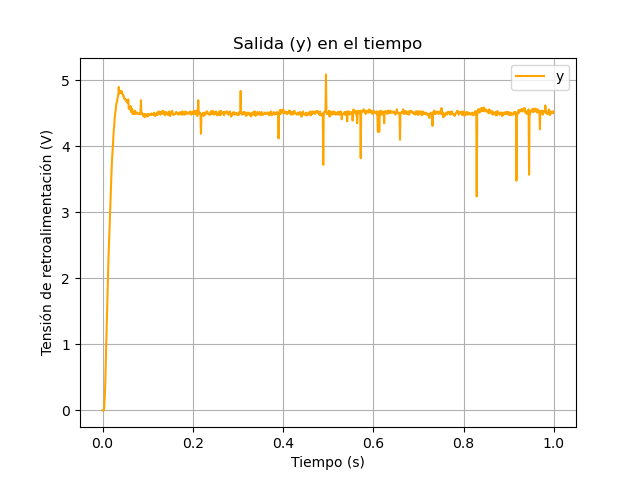
\includegraphics[width=\textwidth]{kalman_altoq_y.png}
        %\vspace{-0.25cm}
        \caption{Señal de salida (Volts).}
        \label{fig:kalman_altoq_y}
    \end{subfigure}
    \begin{subfigure}[b]{0.49\textwidth}
        \centering
        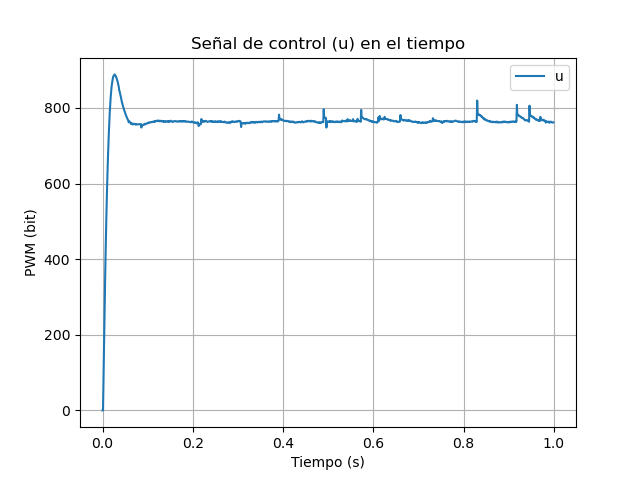
\includegraphics[width=\textwidth]{kalman_altoq_u.png}
        %\vspace{-0.25cm}
        \caption{Señal de control (duty cycle en bits).}
        \label{fig:kalman_altoq_u}
    \end{subfigure}

    \begin{subfigure}[b]{0.49\textwidth}
        \centering
        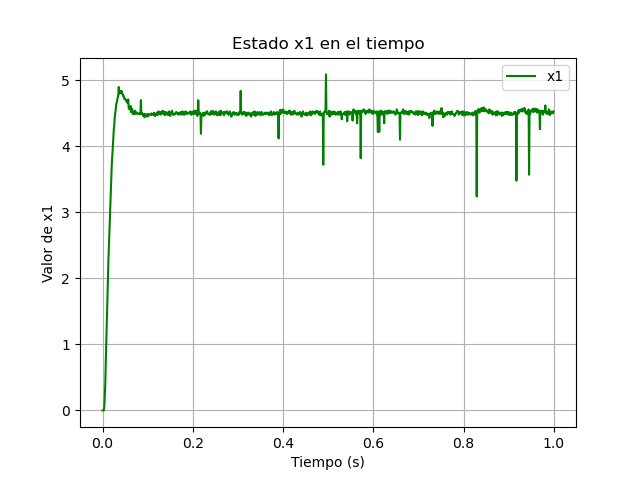
\includegraphics[width=\textwidth]{kalman_altoq_x1.png}
        %\vspace{-0.25cm}
        \caption{Estado estimado x1 (Volts).}
        \label{fig:kalman_altoq_x1}
    \end{subfigure}
    \begin{subfigure}[b]{0.49\textwidth}
        \centering
        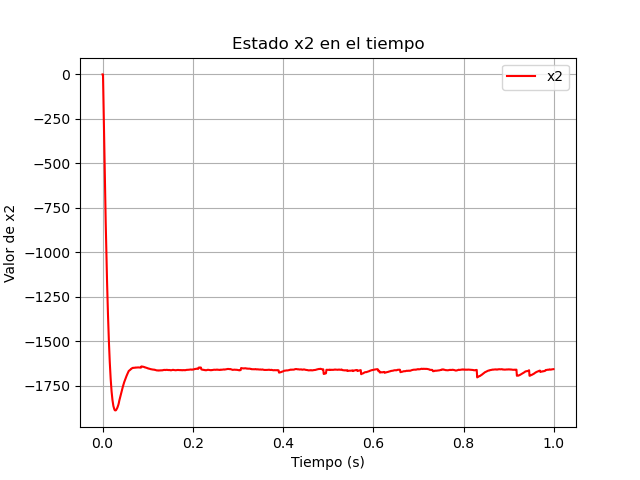
\includegraphics[width=\textwidth]{kalman_altoq_x2.png}
        %\vspace{-0.25cm}
        \caption{Estado estimado x2.}
        \label{fig:kalman_altoq_x2}
    \end{subfigure}

    \vspace{-0.25cm}
    \caption{LQR con integrador y filtro de Kalman. Setpoint = $4.5\ V$. Q = $10^{11}$, R = $10^{-15}$.}
    \label{fig:kalman_altoq}
\end{figure}
\vspace{-0.5cm}

Se observa que, al tener un filtro de Kalman con alto valor de Q, la estimación confía más en la medición de la salida que en la predicción
basada en el modelo. El estado x1 sigue perfectamente a la señal de retroalimentación, incluso aquellos picos provocados por ruido.
Eso causa reacciones indebidas en la señal de control, modificando momentáneamente la señal de salida en el sentido opuesto al ruido.
Sin embargo, el sistema de control es lo suficientemente rápido para volver a la referencia sin problemas.

\begin{figure}[H]
    \centering

    \begin{subfigure}[b]{0.49\textwidth}
        \centering
        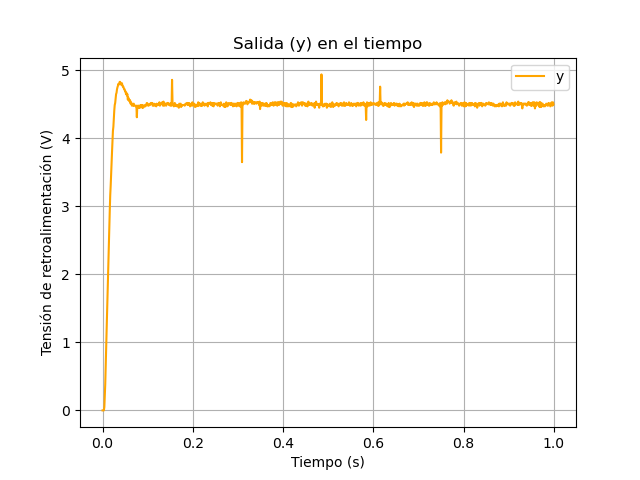
\includegraphics[width=\textwidth]{kalman_altor_y.png}
        %\vspace{-0.25cm}
        \caption{Señal de salida (Volts).}
        \label{fig:kalman_altor_y}
    \end{subfigure}
    \begin{subfigure}[b]{0.49\textwidth}
        \centering
        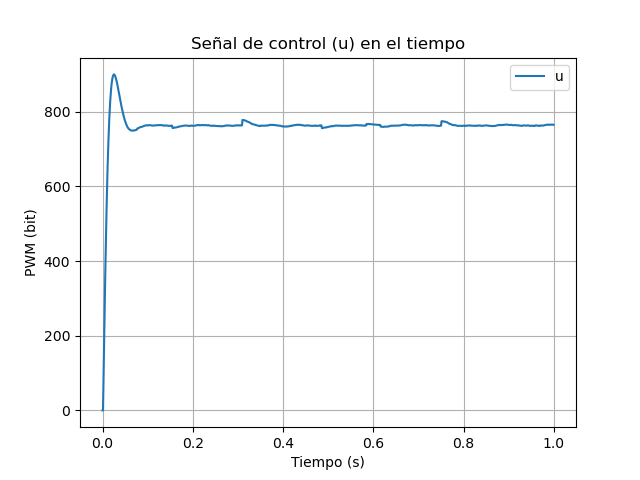
\includegraphics[width=\textwidth]{kalman_altor_u.png}
        %\vspace{-0.25cm}
        \caption{Señal de control (duty cycle en bits).}
        \label{fig:kalman_altor_u}
    \end{subfigure}

    \begin{subfigure}[b]{0.49\textwidth}
        \centering
        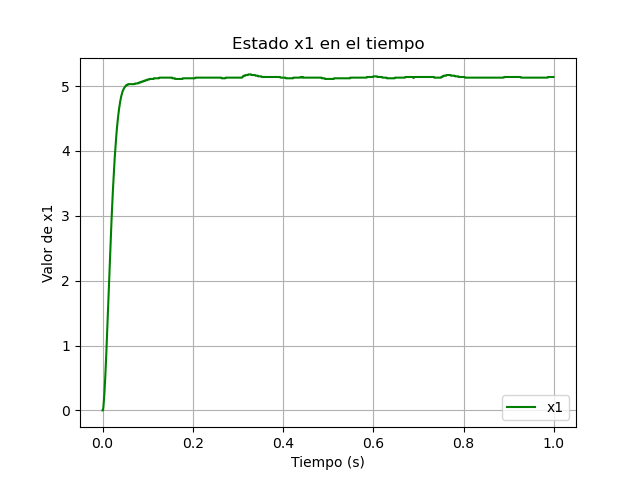
\includegraphics[width=\textwidth]{kalman_altor_x1.png}
        %\vspace{-0.25cm}
        \caption{Estado estimado x1 (Volts).}
        \label{fig:kalman_altor_x1}
    \end{subfigure}
    \begin{subfigure}[b]{0.49\textwidth}
        \centering
        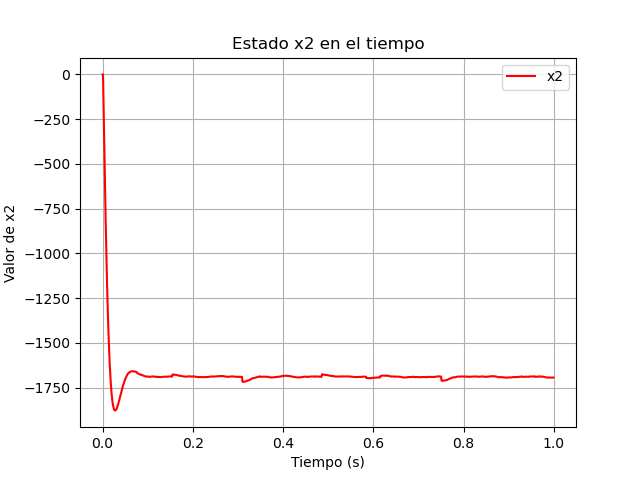
\includegraphics[width=\textwidth]{kalman_altor_x2.png}
        %\vspace{-0.25cm}
        \caption{Estado estimado x2.}
        \label{fig:kalman_altor_x2}
    \end{subfigure}

    \vspace{-0.25cm}
    \caption{LQR con integrador y filtro de Kalman. Setpoint = $4.5\ V$. Q = $10^{-15}$, R = $10^{11}$.}
    \label{fig:kalman_altor}
\end{figure}
\vspace{-0.5cm}

Con un filtro de Kalman con alto valor de R, la estimación confía más en la predicción basada en el modelo que en
la medición. El estado x1 es completamente distinto al de la salida, ya que el modelo no es perfecto. Se observa que los ruidos
presentes en la señal de realimentación no afectan en lo absoluto al estado x1 y, en consecuente, a la señal de control.
Sin embargo, una confianza excesiva en el modelo puede causar problemas al momento de existir perturbaciones en la entrada o salida 
(mayor tiempo de respuesta, oscilaciones, etc.).

Finalmente, se optan por valores intermedios de Q y R para el filtro de Kalman, obteniendo la siguiente respuesta final:

\begin{figure}[H]
    \centering

    \begin{subfigure}[b]{0.49\textwidth}
        \centering
        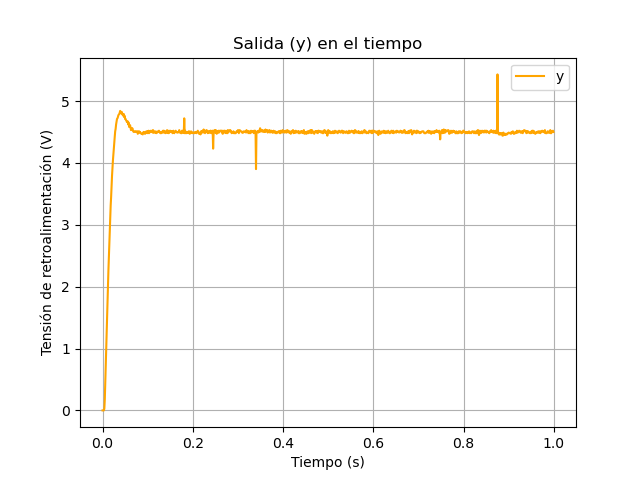
\includegraphics[width=\textwidth]{kalman_final_y.png}
        %\vspace{-0.25cm}
        \caption{Señal de salida (Volts).}
        \label{fig:kalman_final_y}
    \end{subfigure}
    \begin{subfigure}[b]{0.49\textwidth}
        \centering
        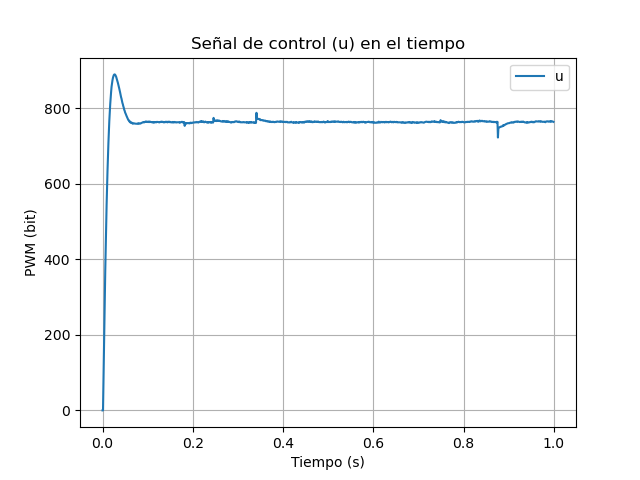
\includegraphics[width=\textwidth]{kalman_final_u.png}
        %\vspace{-0.25cm}
        \caption{Señal de control (duty cycle en bits).}
        \label{fig:kalman_final_u}
    \end{subfigure}

    \begin{subfigure}[b]{0.49\textwidth}
        \centering
        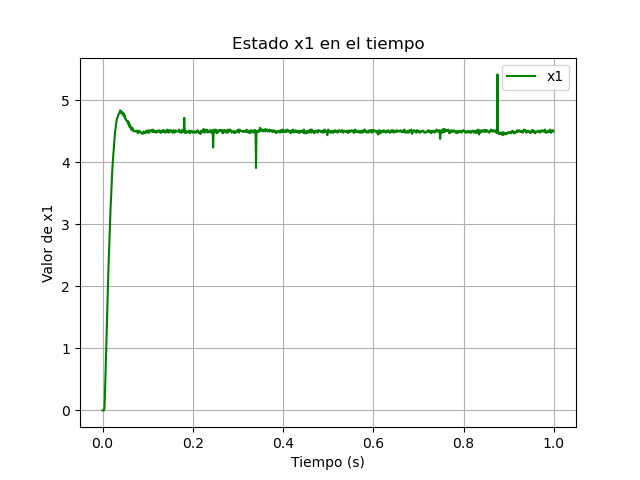
\includegraphics[width=\textwidth]{kalman_final_x1.png}
        %\vspace{-0.25cm}
        \caption{Estado estimado x1 (Volts).}
        \label{fig:kalman_final_x1}
    \end{subfigure}
    \begin{subfigure}[b]{0.49\textwidth}
        \centering
        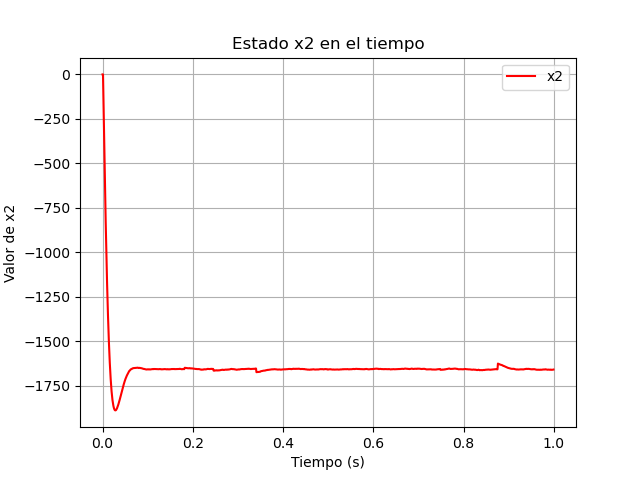
\includegraphics[width=\textwidth]{kalman_final_x2.png}
        %\vspace{-0.25cm}
        \caption{Estado estimado x2.}
        \label{fig:kalman_final_x2}
    \end{subfigure}

    \vspace{-0.25cm}
    \caption{LQR con integrador y filtro de Kalman. Setpoint = $4.5\ V$. Q = $1$, R = $0.01$.}
    \label{fig:kalman_final}
\end{figure}
\vspace{-0.5cm}